\documentclass[conf]{new-aiaa}
%\documentclass[journal]{new-aiaa} for journal papers
\usepackage[utf8]{inputenc}

\usepackage{bbding}


\usepackage{graphicx}
\usepackage{amsmath}
\usepackage[version=4]{mhchem}
\usepackage{siunitx}
\usepackage{longtable,tabularx}
\usepackage{float}
\usepackage{subfigmat}
\usepackage{setspace}
%\doublespacing

\floatstyle{boxed}
\restylefloat{figure}

\setlength\LTleft{0pt} 

\title{Optimized vector field UAV guidance for path following and obstacle avoidance with singularity detection}

\author{Garrett Clem\footnote{Graduate Research Assistant, Mechanical Engineering, 251 Stocker Center}}


\author{Jay P. Wilhelm\footnote{Assistant Professor, Mechanical Engineering, 251 Stocker Center}}
\affil{Ohio University, Russ College of Engineering and Technology, Athens, OH, 45701}




\begin{document}

\maketitle

\begin{abstract}



Unmanned Aerial Vehicles conventionally navigate by following a series of pre-planned waypoints that may have to be re-planned when flying in a dynamic environment or encountering previously unknown obstacles. Waypoints are generally planned off-line and relayed to the UAV, taking up time and autopilot communication resources. Attractive path following and repulsive obstacle avoidance vector fields have been summed together to produce UAV guidance that follows pre-planned paths and avoids obstacles without the need to re-plan. Summing attractive and repulsive vector fields may produce small regions of null guidance, called singularities, which could potentially lead to trap situations. An investigation into singularity mitigation by vector field weight parameterization is presented. 


\end{abstract}



\section{Nomenclature}

{\renewcommand\arraystretch{1.0}
\noindent\begin{longtable*}{@{}l @{\quad=\quad} l@{}}
$UAV$  & Unmanned Aerial Vehicle \\
$VF$   & Vector Field \\
$VFF$  & Virtual Force Field \\
$LVF$  & Lyapunov Vector Field \\
$GVF$  & Goncalves Vector Field \\
$\overrightarrow{X}$  & UAV position \\
$\overrightarrow{U}$  & UAV velocity \\
$\theta$  & UAV heading \\
$\dot{\theta}$  & UAV heading rate \\
$u$  & UAV speed \\
$dt$  & discrete time step\\


$\overrightarrow{V}_{g}$  	 & Total vector guidance\\
$\overrightarrow{V}_{conv}$  & Convergence Vector\\
$\overrightarrow{V}_{circ}$  & Circulation Vector\\

$G$  & Convergence Weight\\
$H$  & Circulation Weight\\
$V$  & Potential Function\\

$r_O$  & Obstacle Radius\\
$R$  & Decay Radius\\
$\gamma$  & Path Deviation Cost\\
$\alpha_i$  & Surface Function\\

$x$  & UAV horizontal position\\
$y$  & UAV vertical position\\

$x_c$  & Circular obstacle horizontal position\\
$y_c$  & Circular obstacle vertical position\\

$d$  & Range to obstacle\\

$P$  & Obstacle Decay Weight\\
$n$  & Number of spatial dimensions\\
$\delta$  & Target path angle \\
$||\bullet || $  & Vector magnitude \\
$m$  & Obstacle radius multiplier \\
$k$  & Decay field radius multiplier \\




\end{longtable*}}

\section{Introduction}


%Paths have already been deemed to meet mission requirements
%Avoiding obstacles while minimizing deviation from the prescribed path would be benefitial
%Planning missions (path connecting sequential tasks)
%Following path with waypoints
%
%
%There are many methods for planning obstacle free and flyable paths, however in general the methods can be simplified into two steps consisting of optimization and path refinement. Optimization determines the least cost straight line path which is further refined to ensure the path is flyable.
%
%INTRODUCTION TO UAVS


%Unmanned Aerial Vehicles (UAV)s are pilotless aircraft used by military, police, and civilian communities for tasks such as reconnaissance, damage assessment, surveying, and target tracking \cite{ariyur_autonomous_2008,teuliere_chasing_2011}. Many of these tasks depend on the UAVs ability to autonomously follow a pre-planned path while potentially avoiding obstacles. Pre-planned paths are typically generated on a remote ground station and relayed to the UAV’s autopilot. On-board guidance systems attempt to minimize the lateral error to the path by commanding a heading pointing to the path. Guidance methods for following a pre-planned path include geometric methods such as waypoint or carrot chasing and control techniques such as proportional-integral-derivative (PID), non-linear guidance laws, and linear quadratic regulator (LQR) \cite{sujit_unmanned_2014}. Due to traditional guidance method's dependence on a path planner to construct an obstacle free and flyable path, these methods often lack a mechanism to avoid obstacles unknown during planning. Re-planning and relaying a new obstacle free path may be impossible under certain conditions, such as flying beyond line-of-sight. Path planning on-board to avoid a new obstacle could be accomplished by inserting a new temporary path or by completely re-planning, however introduces several challenges such as waypoint placement and density. \\
%
%Additional methods for avoiding obstacles in real time include potential field \cite{borenstein_real-time_1990,borenstein_vector_1991} and vector field \cite{frew_cooperative_2007,griffiths_vector_2006,goncalves_artificial_2009,goncalves_circulation_2010,goncalves_vector_2010} which employ the use of artificial attractive and repulsive forces to pull a UAV towards a goal while pushing away from nearby obstacles. Potential field has been used as a path planner and guidance system in obstacle rich environments, however potential field suffers from several limitations including local minima, oscillations, and may cause excess deviation from the desired path. Vector field guidance (VFG) converges and circulates a pre-defined path and may be summed with additional repulsive vector fields to produce an obstacle avoidance. Each field's behavior can be modified by weighting convergence, circulation, and time-varying components by multiplicative scalars. Previous investigations into vector field obstacle avoidance only considered negative static weights for convergence which did not aid in circumnavigating an obstacle and can introduce conditions which lead to guidance singularities. Further optimization of vector fields decay radii and circulation weights may produce an improved avoidance guidance while also removing singularities from the UAVs route. \\
%
%The contribution of this study is to demonstrate a vector field parameter optimization method for determining decay radius and circulation weights for a real-time guidance that circumnavigates obstacles which lie along a pre-planned path while also removing singularities from the UAVs route. A method for determining obstacle decay radius, circulation, and repulsion such that a UAV avoids obstacles while minimizing deviation from the planned path is presented. The modified guidance will then be compared against waypoint, Potential Field, and un-modified path following guidance in simulation for cross track error from planned path.\\
%
%============================================\\
Unmanned aerial vehicles (UAV)s are pilotless aircraft used by military, police, and civilian communities for tasks such as damage assessment \cite{fernandez_galarreta_uav-based_2015}, surveying \cite{remondino_uav_2012}, and target tracking \cite{frew_cooperative_2007,oh_coordinated_2013,hyondong_oh_coordinated_2015,oliveira_moving_2016}. Many UAV tasks depend on the vehicle's ability to autonomously follow a mission path while potentially avoiding obstacles and no-fly zones. Flight paths are typically followed by implementing guidance systems such as waypoint \cite{osborne_waypoint_2005}, proportional-integral-derivative (PID) \cite{rhee2010tight}, non-linear guidance laws \cite{park2007performance}, or linear quadratic regulator (LQR) \cite{ratnoo_adaptive_2011}. Conventional path following guidance systems are typically not capable of avoiding obstacles without partially or completely re-planning the path. Paths are typically generated on a remote ground station and relayed to the UAV’s autopilot. Updating a mission may be impossible under certain conditions, such as flying outside of communication range. Avoiding obstacles without path re-planning has been achieved with potential field \cite{borenstein_real-time_1990,borenstein_vector_1991} and vector field \cite{frew_cooperative_2007,griffiths_vector_2006,goncalves_artificial_2009,goncalves_circulation_2010,goncalves_vector_2010} guidance methods.\\

 Potential field employs the use of artificial attractive and repulsive forces that direct a UAV towards a goal while locally pushing away from nearby obstacles \cite{khatib_real-time_1986}. Potential field may cause excess deviation from the desired path and provides guidance for converging to a singular point \cite{borenstein_real-time_1990,borenstein_vector_1991} which is not ideal for fixed wing UAVs. Another method that uses attractive and repulsive forces, Gradient Vector Field (GVF), provides a continuous heading guidance that directs a UAV to converge and follow an arbitrary path that lies at the intersection of surfaces \cite{goncalves_artificial_2009,goncalves_circulation_2010,goncalves_vector_2010}. \\

GVF's may consist of decoupled convergence and circulation terms that can be weighted by scalars to influence field strength and direction. Negating convergence weights can produce a repulsive GVF that pushes away from a path. Obstacles may be avoided by summing together attractive path following and repulsive obstacle fields. Determining circulation and obstacle field decay radius to minimize deviation from a planned path while avoiding guidance singularities is the contribution of this research. The optimized GVF guidance method will be compared for path deviation against both waypoint and potential field methods for a worst=case head on collision scenario. 



%The GVF method was modified in the standoff tracking scenario presented in [wwc] where a fixed wing UAV was tasked with tracking a slower moving ground target while avoiding static obstacles. An attractive circular GVF was attached to the moving ground target which guided the fixed wing UAV to enter a loiter orbit around the target. Circular repulsive vector fields were attached to the static obstacles and summed with the attractive GVF. The repulsive GVFs pushed the UAV away from keep-out zones while allowing the UAV to return to the desired loiter path. \\







%Unmanned Aerial Vehicles (UAV)s are pilotless aircraft used by military, police, and civilian communities for tasks such as reconnaissance, damage assessment, surveying, and target tracking \cite{ariyur_autonomous_2008,teuliere_chasing_2011}. Tasks can be performed by a single UAV or cooperate with a team of other air, ground, or marine vehicles \cite{oh_coordinated_2013,hyondong_oh_coordinated_2015,ulun_coordinated_2013}. UAVs are ideal for remote data collection due to their low cost, endurance, and reduced risk to human life. Data can be collected by loitering the aircraft around an area of interest (AOI) or along a sensor path, such as a road or tree-line. Missions for collecting data are typically pre-planned on a remote ground station where an obstacle free and flyable path is generated. Typically paths are deconstructed into a series of discrete waypoints that the UAV navigates to through the use of a line-of-sight guidance. While navigating the pre-planned path previously unknown obstacles may be discovered and a new obstacle free path may have to be generated, which may be difficult or impossible if the UAV is out of radio range. Additional methods for avoiding obstacles in real time include potential field and vector field which employ the use of artificial attractive and repulsive forces to pull a UAV towards a goal while pushing away from obstacles. Potential field is a popular solution to both path planning and guidance problems in obstacle rich environments, however suffers from several limitations including local minima, oscillations, and may cause excess deviation from the desired sensor line. Vector field guidance converges and circulates a pre-defined path and may be summed with additional repulsive vector fields to produce an obstacle avoidance. Previous methods only considered repulsive fields which do not aid in circumnavigating an obstacle and also introduce conditions which may lead to vector field singularities. \\
%
% Further optimization of vector fields to include circulation may produce an efficient real-time guidance for avoiding obstacles while also removing singularities from the UAVs path. A method for determining obstacle decay radius, circulation, and repulsion such that a UAV avoids obstacles while minimizing path deviation is presented. The modified guidance will then be compared against waypoint, Potential Field, and un-modified path following guidance in simulation for cross track error and deviation from sensor path. Lastly, the optimized vector field will then be demonstrated on a crazyflie 2.0 multi-rotor simulating fixed wing constraints. 

\section{Literature}
Remaining close to a planned path is essential for safe and efficient operation of UAVs. Obstacles or no-fly zones that are discovered after a path has been planned would traditionally require that a new obstacle free and flyable path be recalculated and relayed to the UAV. These paths are commonly represented as a series of finite waypoints in commercial UAV autopilots such as the Piccolo \cite{piccolo}, Kestral \cite{kestrel}, and Pixhawk \cite{pix}. The on-board autopilot aligns the vehicle with the current active waypoint and switches to the subsequent waypoint once the UAV has reached a defined distance from the waypoint’s center, referred to as the waypoint radius. \\

Avoiding obstacles with waypoint guidance may be accomplished by creating diversion waypoints off the planned path and outside of the obstacle \cite{goerzen_survey_2010}. A single diversion waypoint may be enough to direct the UAV away from the obstacle, however may result in excess deviation from the planned path. Increasing the number of deviation waypoint may allow for the UAV to travel more of the planned path prior to deviating to avoid the obstacle. When it is not possible to plan a new obstacle free path, such as when the UAV is not able to communicate with the ground station, it may be beneficial to use a guidance system that can avoid obstacles without the path re-planning. Methods for obstacle avoidance guidance can be found in potential field \cite{borenstein_real-time_1990,borenstein_vector_1991} and vector field guidance \cite{frew_cooperative_2007,nelson_cooperative_2005,nelson_vector_2006,nelson_vector_2007,griffiths_vector_2006,goncalves_artificial_2009,goncalves_circulation_2010,goncalves_vector_2010}. \\ 


%\begin{figure}[H]
%	\begin{subfigmatrix}{2}% number of columns
%		\centering	
%		\subfigure []{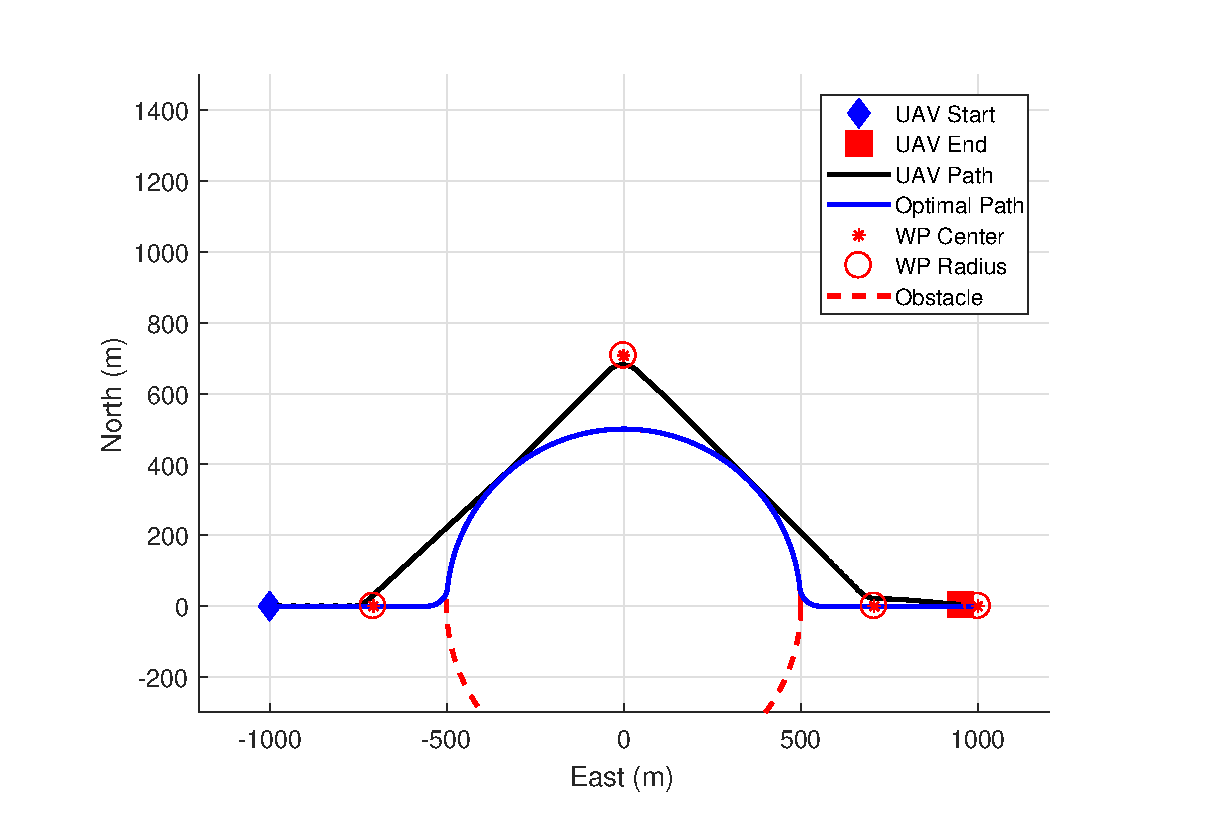
\includegraphics[width=8cm,trim=40 0 60 0,clip] {Figures/Waypoints/1Wpts}}
%		\subfigure []{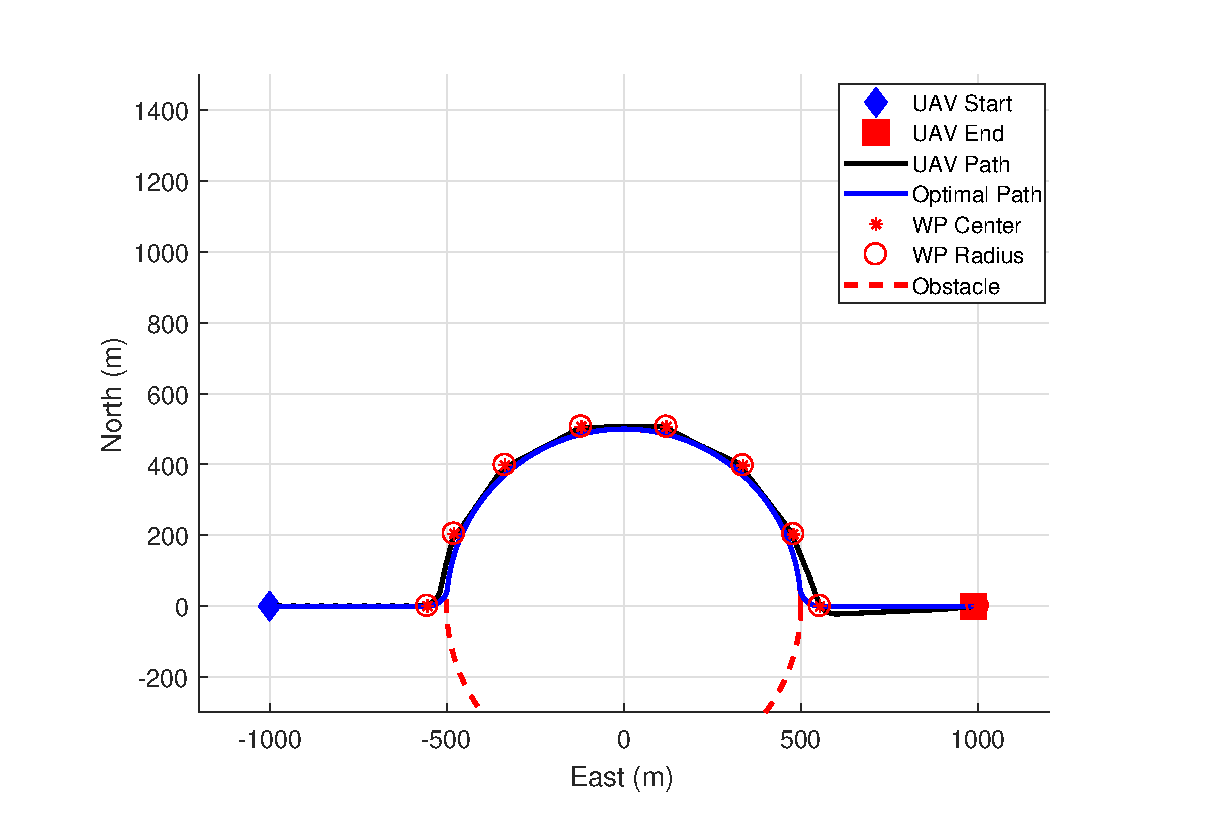
\includegraphics[width=8cm,trim=40 0 60 0,clip] {Figures/Waypoints/6Wpts}}
%		\hspace*{0mm}
%	\end{subfigmatrix}
%	\caption{Obstacle Diversion Waypoints}
%	\label{fig:numWaypointsPath}
%\end{figure}
%
%Determining the number of diversion waypoints to avoid a circular obstacle to minimize the deviation from a planned path can be accomplished by observing the change in a function cost $\gamma$ with respect to the number of waypoints, Equation \ref{eq:diversionCost}. The cost function is scaled and non-dimensionalized by diving by the obstacles radius $r_o$. As the number of waypoints increase around the obstacle the decrease in cost begins to have diminishing returns and approaches an asymptote, shown in Figure \ref{fig:numWaypoints}. 
%
%
%\begin{equation}
%\label{eq:diversionCost}
%\begin{aligned}
%\gamma =  \frac{1}{r_O}\int_{0}^{tf}ydt
%\end{aligned}
%\end{equation}
%
%\begin{figure}[H]
%	\centering
%	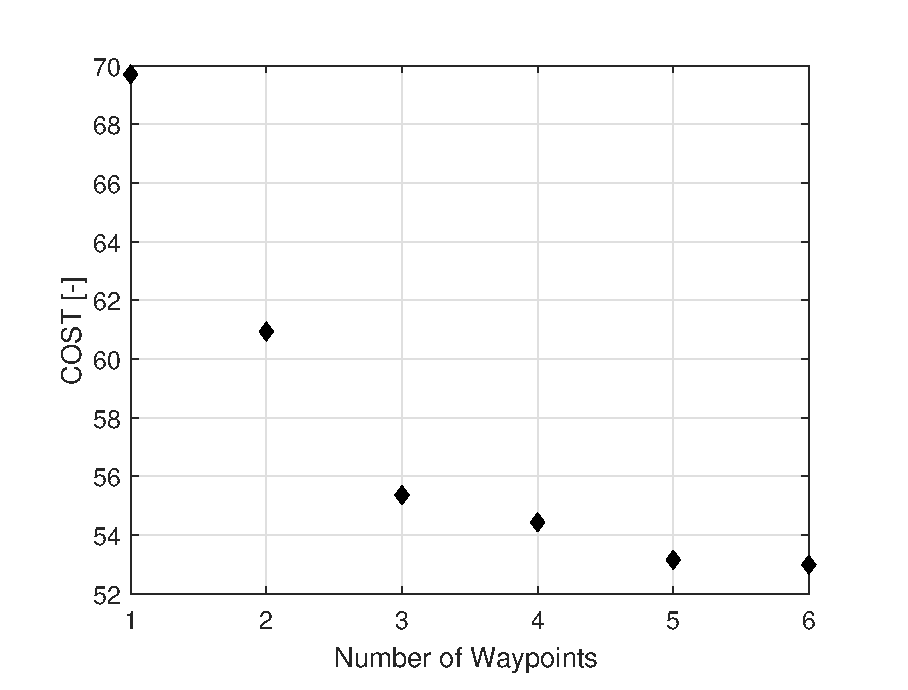
\includegraphics[width=10cm]{Figures/Waypoints/costVnumWpts}
%	\caption{Cost impact versus number of waypoints}
%	\label{fig:numWaypoints}
%\end{figure}



Potential field is based on the principle of artificial attractive and repulsive forces acting on a point mass to guide a system to a desired goal while avoiding static and dynamic obstacles \cite{khatib_real-time_1986}. Goals are represented as an attractive force that pull a point mass in the direction of minimal energy while obstacles are represented as repulsive forces that act locally to push the point mass away. Potential field is also capable of acting as a path and trajectory planning algorithm \cite{rimon_exact_1992}, possibly eliminating the off-board path planner. An example of potential field can be found in \cite{borenstein_real-time_1990,borenstein_vector_1991,koren_potential_1991} which allowed for real time goal seeking with obstacle avoidance on a mobile ground robot equipped with ultrasonic sensors. The robot was attracted towards a goal with constant magnitude force. In the immediate area of the robot, an active window exists which records integer certainty values inside discrete cells. Cells containing an obstacle provide a repulsive force opposite in direction to the line-of-sight from vehicle to cell location. The total repulsive force exerted on the robot is determined by summing the active cells. Summing together attractive and repulsive forces produce a vector that can be used for heading guidance. \\

%\begin{equation}\label{eq:vffGoal}
%\overrightarrow{F_t} = F_{ct} \bigg( \frac{x_t-x_0}{d_{t}}\hat{x} + \frac{y_t-y_0}{d_{t}}\hat{y}\bigg)
%\end{equation}
%
%\begin{equation}\label{eq:vffRepulse}
%\overrightarrow{F_{i,j}} = \frac{F_{cr}W^nC_{i,j}}{d^n_{i,j}} \bigg( \frac{x_i-x_0}{d_{i,j}}\hat{x} + \frac{y_i-y_0}{d_{i,j}}\hat{y}\bigg)
%\end{equation}

%The total repulsive force exerted on the robot is determined by summing the active cells, shown in Equation \ref{eq:vffRepulseSum}
%
%
%\begin{equation}\label{eq:vffRepulseSum}
%\overrightarrow{F_r} = \sum_{i,j}\overrightarrow{F_{i,j}}
%\end{equation}




%Summing together attractive and repulsive forces produce a vector $\overrightarrow{R}$ that can be used for heading guidance, shown in Equation \ref{eq:vffHeading}.

%\begin{equation}\label{eq:vffHeading}
%\overrightarrow{R} = \overrightarrow{F_r} + \overrightarrow{F_t}
%\end{equation}

Major drawbacks to potential field were identified in \cite{koren_potential_1991} consisting of local minimum and oscillations in corridors. The local minimum problem occurs when closely spaced obstacle's potential combine to produce a well on the descent gradient where a pre-mature stable point is reached. Proposed solutions to local minimum include object clustering and virtual waypoint method \cite{liu_virtual-waypoint_2016}, virtual escaping route \cite{kim_escaping_2009}, and use of navigation functions \cite{goerzen_survey_2010}. Oscillations in potential field were addressed in \cite{lei_tang_novel_2010} and \cite{li_efficient_2012}. In addition to local minimum and oscillations, potential field may not be ideal for providing guidance to return to a sensor path after avoiding an obstacle. Once the obstacle has been avoided, the attractive goal will direct the UAV in a straight path which may not lie along the sensor line. Guidance that follows an explicit path, deviates when necessary to avoid obstacles, and return back to the explicit path quickly can be accomplished with path following vector fields.  \\


%\subsection{Vector Field Guidance}

Vector fields produce continuous heading guidance that can asymptotically converge and circulate a path. A comparison between vector field and waypoint guidance techniques was presented in \cite{sujit_unmanned_2014} where each method was evaluated based on its complexity, robustness, and accuracy. The vector field model produced guidance that was both robust to external wind disturbances while maintaining a low cross track error. The two most prominent methods for generating vector fields in literature consist of the Lyapunov Vector Field (LVF) \cite{nelson_cooperative_2005,nelson_vector_2006,nelson_vector_2007,frew_cooperative_2007,miao_orthogonal_2016,griffiths_vector_2006} and Gradient Vector Field (GVF) \cite{goncalves_artificial_2009,goncalves_circulation_2010,goncalves_vector_2010,gerlach_autonomous_2014} method. LVFs for converging and following straight and circular paths were described in \cite{nelson_cooperative_2005}. Straight and circular path vector fields can be selectively activated throughout flight to form more complex paths, shown in \cite{nelson_cooperative_2005,nelson_vector_2006,nelson_vector_2007,jung_unmanned_2016}. LVF for curved path following was presented in \cite{griffiths_vector_2006} which may allow for more complex paths and eliminates the need to switch between vector fields. \\

%\subsection{GVF}
The Gradient Vector Field (GVF) method produces a similar field to LVF, however has several advantages over LVFs. GVF produces an \textit{n}-dimensional vector field that converges and circulates to both static and time varying paths, which may be useful for tracking dynamic paths or avoiding dynamic obstacles. Additionally, convergence, circulation, and time-varying terms that make up the GVF are decoupled from each other allowing for easy weighting of the total field. GVFs converge and circulate at the intersection, or level set, of $n-1$ dimensional implicit surfaces ($\alpha_i:\mathbb{R}^n\rightarrow\mathbb{R} | i=1,...,n-1$). The integral lines of the field are guaranteed to converge and circulate the level set when two conditions are met: $1)$ the implicit surface functions are positive definite and $2)$ have bounded derivatives. %Consider the space with dimensions in set \textbf{q}:

%The Goncalves Vector Field (GVF) method for producing vector fields has several advantages over the Lyapunov vector field generation methods.


%\begin{equation}
%\mathbf{q} = \begin{bmatrix} x_1, x_2, ..., x_{n}\end{bmatrix}
%\end{equation}

\noindent
The total vector field for a time invariant path $\overrightarrow{V}$ is calculated by:
\begin{equation}\label{eq:GVF}
\overrightarrow{V} = G \nabla V + H \wedge_{i=1}^{n-1}\nabla\alpha_i
\end{equation}

\noindent
or in component form:

\begin{equation}\label{eq:simpleGVF}
\overrightarrow{V} = G\overrightarrow{V}_{conv} + H\overrightarrow{V}_{circ} 
\end{equation}	

\noindent
where $\overrightarrow{V}_{conv}$ produces vectors that converge to the path and $\overrightarrow{V}_{circ}$ produces vectors that circulate the path. The multiplicative factors $G$ and $H$ are scalar weights to influence the strength of each field component.

\noindent
Convergence is calculated by:

\begin{equation}
% Total field with Conv, Circ, and Time
\overrightarrow{V}_{conv} = \nabla V  
\label{convOnly}
\end{equation}
\noindent
where the potential function $V$ is:

\begin{equation}
V = -\sqrt{{\alpha_1}^2 + {\alpha_2}^2}
\end{equation}

\begin{equation}
\label{eq:gradV}
\nabla V =\begin{bmatrix}
\frac{dV}{dx} \\
\frac{dV}{dy} \\
\frac{dV}{dz}
\end{bmatrix}
\end{equation}


\noindent
Circulation is calculated by taking the wedge product of the gradients of the surface functions:

\begin{equation}
% Total field with Conv, Circ, and Time
\overrightarrow{V}_{circ} =  \wedge_{i=1}^{n-1}\nabla\alpha_i 
\label{circOnly}
\end{equation}

\noindent
In the case of $(n=3)$ spatial dimensions the wedge product simplifies as the cross product:

\begin{equation}
% Total field with Conv, Circ, and Time
\overrightarrow{V}_{circ} =  \nabla\alpha_1 \times \nabla\alpha_2 
\label{circOnlySimp}
\end{equation}


GVFs were used as a heading guidance in \cite{gerlach_autonomous_2014} to direct a Dubin's fixed wing UAV to an arbitrary path. Unlike the GVFs in \cite{goncalves_artificial_2009,goncalves_circulation_2010,goncalves_vector_2010}, the vector field was normalized and the scalars scalars $G$ and $H$ were used as a high level specification of field behavior. Normalizing the field and using scalars to specify field behavior may allow for the field to be modified to provide repulsive vectors and modified path following characteristics, such as how quickly a UAV converges to a path. A vector field that guides a UAV to follow a path, $\overrightarrow{V}_{path}$, may be summed with a repulsive vector field, $\overrightarrow{V}_o$, and weighted by a decay function, $P$, to provide a path following and obstacle avoidance guidance shown in Equation \ref{eq:totalGuidanceObstacleLit}.

\begin{equation}
\label{eq:totalGuidanceObstacleLit}
\overrightarrow{V}_g = \overrightarrow{V}_{path} + P\overrightarrow{V}_{o}
\end{equation}

Summing together path following and obstacle GVFs presents two immediate problems consisting of obstacle field weight selection and the presence of GVF singularities where the two fields cancel. The presence of singularities were mentioned briefly in \cite{nelson_cooperative_2005} and observed in \cite{panagou_motion_2014}. For fixed wing UAVs the lack of guidance may prevent the UAV from avoiding an obstacle, while multi-rotor UAVs may end up in a trap situation where the UAV is guided to a singular point. Methods for detecting singularities in a summed GVF guidance and selecting repulsive field decay radius and circulation weights for an optimized circular obstacle avoidance is the contribution of this research. The improved GVF guidance is shown to have an improved performance over waypoint guidance and potential field without the need re-plan mission paths. 

\subsection{Dubins Model}
Simulating a fixed wing UAV without modeling the high order and non-linear dynamics has been achieved with the Dubin's car model \cite{frew_cooperative_2007,griffiths_vector_2006,nelson_cooperative_2005,nelson_vector_2006,nelson_vector_2007}. It is assumed that the autopilots control system is capable of maintaining stability, speed $u$, and can turn the vehicle at a maximum fixed turn rate $\dot{\theta}$. The position of the UAV $\overrightarrow{X}$ at time $t$ is calculated from the integral of the velocity vector $\overrightarrow{U}$, Equation \ref{eq:uavPosition}. Heading is an input from a guidance system, such as waypoint, potential field, or vector field.

\begin{equation}
\label{eq:uavVelocity}
\overrightarrow{U}(t) = u \begin{bmatrix}
cos(\theta(t)) \\
sin(\theta(t))
\end{bmatrix}
\end{equation}


\begin{equation}
\label{eq:uavPosition}
\overrightarrow{X}(t) = \overrightarrow{U}dt + \overrightarrow{X}(t-1)
\end{equation}


\begin{equation}
\label{turnRate}
\dot{\theta} \leq 20 deg/s
\end{equation}


%\section{Optimal Path}
%\begin{equation}\label{eq:optPath}
%y = \frac{u}{\dot{theta}} \newline
%\end{equation}
%
%\begin{equation}\label{eq:optPath}
%X = obstX - \sqrt{(turnR-obstR)^2-(y-obstY)^2}
%\end{equation}
%
%\begin{equation}\label{eq:optPath}
%\Theta = \sin^{-1}\Bigg(\frac{y-obstY}{obstR+turnR}\Bigg)
%\end{equation}
%
%\begin{equation}\label{eq:optPath}
%\beta = \Big[\frac{3\pi}{2},\pi-\Theta\Big]
%\end{equation}
%
%\begin{equation}\label{eq:optPath}
%\gamma = \Big[\pi-\Theta,\Theta\Big]
%\end{equation}
%
%\begin{equation}\label{eq:optPath}
%\zeta = \Big[\pi+\Theta,\frac{30pi}{2}\Big]
%\end{equation}
%
%\begin{equation}\label{eq:optPath}
%x = 
%\begin{cases} 
%0 & X+turnR*cos(beta) \\
%\frac{100-x}{100} & obstX + obstR*cos(gamma) \\
%0 & -X+turnR*cos(zeta) 
%\end{cases}
%\end{equation}



% For highly uncertain or dynamic environments, path planning may have to occur frequently which increases communication overhead for the autopilot
%
%% The state of the environment would then need to be transmitted back to the ground station and a new optimized and refined path be generated along with a series of waypoints. 
%%
%%
%%
%%During waypoint navigation the UAV may encounter obstacles or environmental changes that would require a new set of obstacle free waypoints to be generated. 
%
%
%For highly uncertain or dynamic environments, there may have to be frequent updates which increases the communication overhead of the autopilot since paths may be updated and communicated from the ground. Additionally, if communication is delayed or lost, waypoints may not be updated rapidly enough and the UAV may fail to avoid the obstacles if the autopilot is following outdated waypoints that violate an obstacle. Real time obstacle avoidance without the need to replan may be found in the use of potential and vector fields, which operate on the principle of artificial attractive and repulsive forces to guide a robotic system. 






\section{Methods}
Optimizing GVF obstacle decay radius and circulation weight for minimizing deviation from a planned path and detecting GVF singularities was the objective of this research. Guidance for converging and following a straight path using GVF is presented along with the effects of modifying path circulation weights. A circular obstacle is represented as a repulsive GVF and summed with path following guidance. The contribution of this work is to present singularity detection in the summed field with strictly repulsive GVF obstacle and compared to an obstacle field with circulation. Additionally, A method for selecting GVF decay radius and circulation for an optimized obstacle avoidance is presented. Lastly, simulations comparing the improved GVF guidance to waypoint and potential field is shown. 


\subsection{Optimal Avoidance Route for Straight Path}
Route around obstacles can be computed by a number of methods discussed in \cite{goerzen_survey_2010}. To evaluate the performance of the optimized GVF developed in this work in terms of path deviation, a geometrically optimal route around a circular obstacle was developed. The path for avoiding a circular obstacle while maximizing the sensor path coverage can be accomplished with three circular arc turns. The circular obstacle is defined to have a radius $R$ and a lateral distance $Y_0$ from the sensor path in frame $I$. The first and third arc utilize the UAVs minimum turning radius, $\theta_r$, calculated in Equation \ref{eq:turnRadius}. The start of the first minimum radius turn begins when the UAV's horizontal position $x$ reaches  $\tilde{x}$ from the path frame origin. At a horizontal position $-\hat{x}$ the UAV turns with a radius of the obstacle $R$ and exits when the UAVs horizontal position reaches $\hat{x}$. 

\begin{equation}
\label{eq:turnRadius}
\theta_r = \frac{u}{\dot{\theta}}
\end{equation}

The horizontal points $\tilde{x}$ and $\hat{x}$ are shown in Equations \ref{eq:optPathXtilde} and \ref{eq:optPathXhat} respectively. 

\begin{equation}
\label{eq:optPathXtilde}
\widetilde{x} = -\sqrt{(\theta_r+R)^2 - (\theta_r-Y_o)^2}
\end{equation}

\begin{equation}
\label{eq:optPathXhat}
\hat{x} = \frac{R\sqrt{(r+R)^2-(\theta_r-Y_o)^2}}{R+\theta_r}
\end{equation}

The avoidance path for navigating around a circular obstacle with maximum coverage of a sensor line is defined in Equation \ref{eq:optPath} and shown in Figure \ref{fig:optimalpath}.


\begin{equation}
\label{eq:optPath}
y(x) = \left\{
\begin{array}{ll}
\widetilde{y} -\sqrt{\theta_r^2 - (x-\widetilde{x})^2} &  x < -\hat{x} \\
Y_o +\sqrt{R^2 - x^2} & -\hat{x} \leq x \geq \hat{x}\\
\widetilde{y} -\sqrt{\theta_r^2 - (x+\widetilde{x})^2}&  x > -\hat{x}
\end{array}
\right.
\end{equation}

\begin{figure}[H]
	\centering
	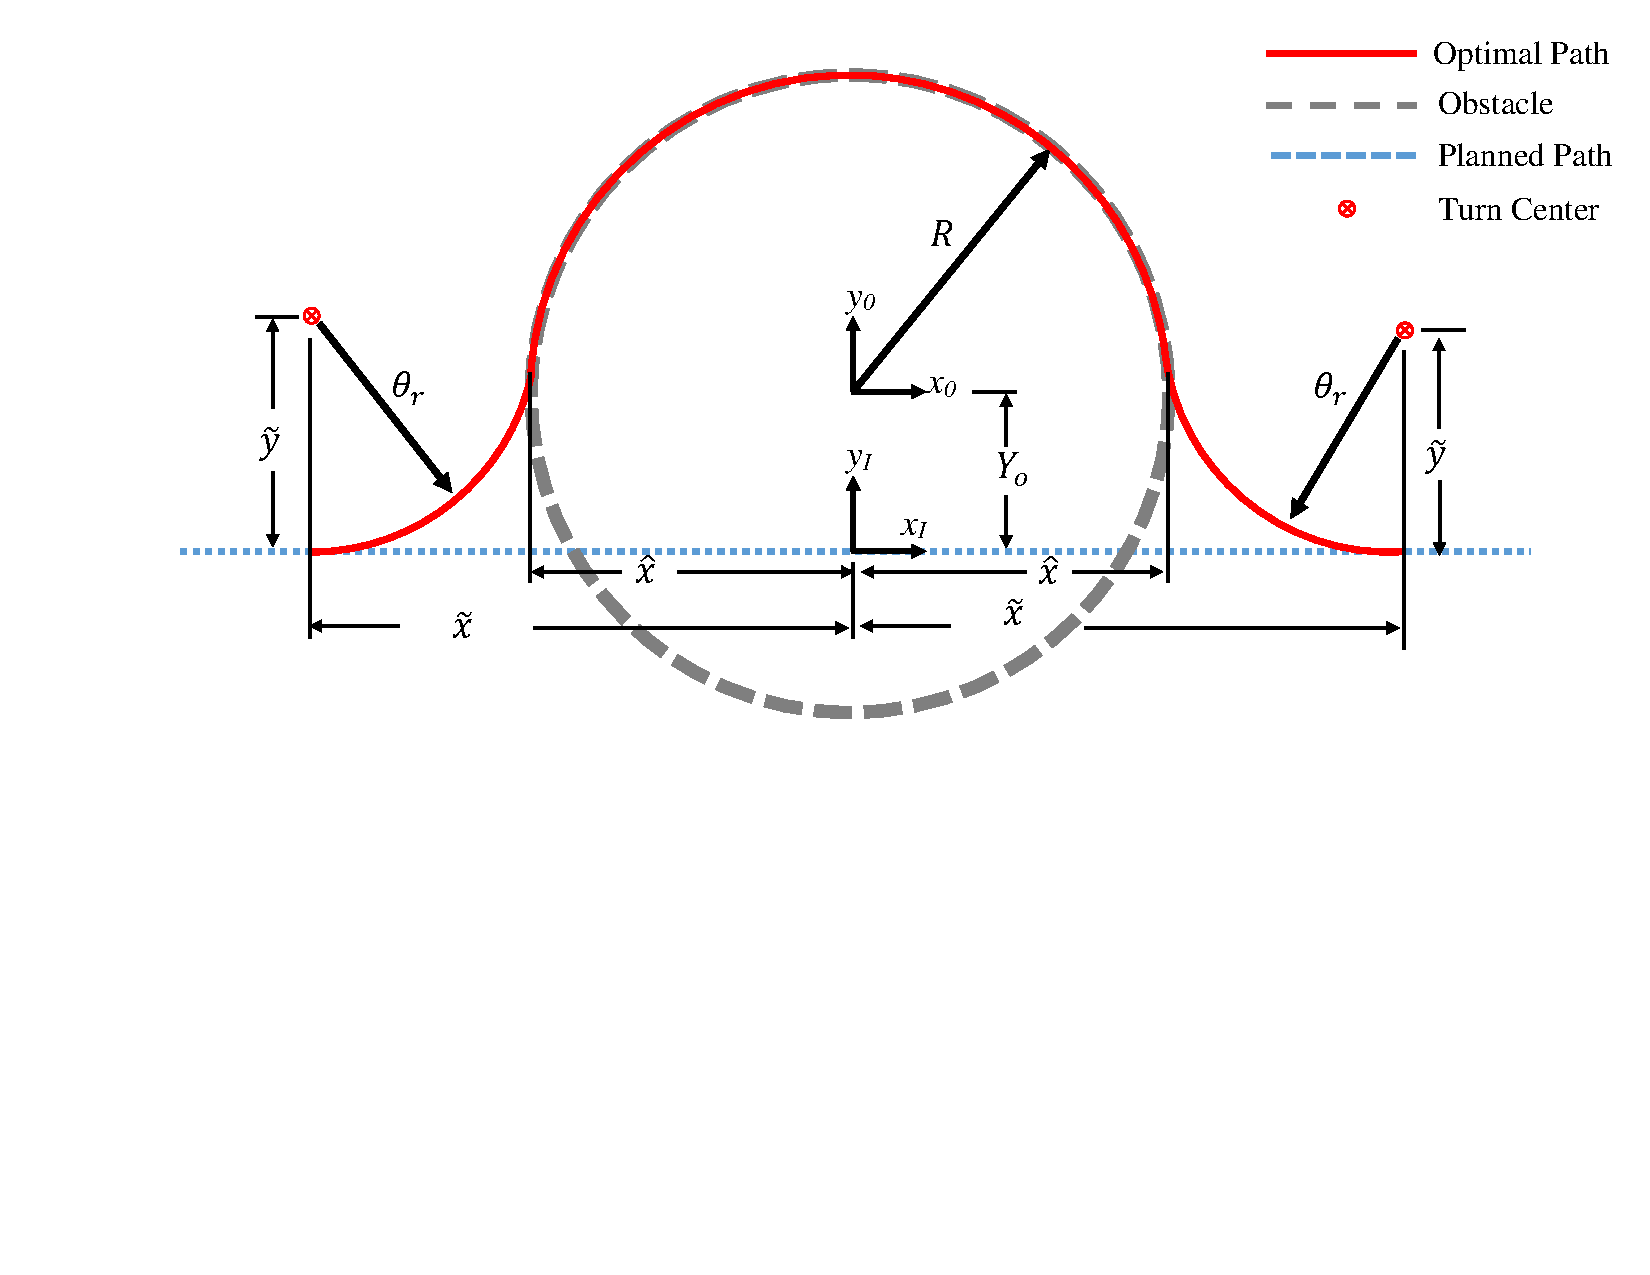
\includegraphics[width=0.7\linewidth ,trim=0 265 0 20,clip,width=15cm]{Figures/optimalPath/optimalPath}
	\caption{Optimal Kinematic Path Around Circular Obstacle}
	\label{fig:optimalpath}
\end{figure}




\subsection{Path Following with GVF}

Straight path following guidance of a time invariant line for a planar UAV at position $(x,y)$ is achieved by summing together convergence $\overrightarrow{V}_{conv}$ and circulation $\overrightarrow{V}_{circ}$ terms shown in Equation \ref{eq:simpleGVF}. The GVF converges and circulates at the intersection of two implicit surfaces, and for a straight path those surfaces are represented by planes. The implicit surface function $\alpha_1$ is at angle $\delta$ with respect to the x-axis and plane $\alpha_2$ is at constant height of $z$, which is the desired altitude, shown in Equations \ref{eq:pathFunction} and \ref{eq:pathFunctionZ} respectively, and the surfaces in Figure \ref{fig:planeIntersection}.


\begin{equation}
\label{eq:pathFunction}
\alpha_1 = cos(\delta)x + sin(\delta)y
\end{equation}

\begin{equation}
\label{eq:pathFunctionZ}
\alpha_2 = z
\end{equation}

\noindent
The gradient potential, $\nabla V$ is shown in Equation \ref{eq:potentialFunctionGrad}.

\begin{equation}
\label{eq:potentialFunctionGrad}
\nabla V = -\frac{1}{2(\sqrt{\cos^2(\delta) x^2+2\cos(\delta)\sin(\delta) xy +\sin^2 (\delta) y^2})} \begin{bmatrix}
2x\cos^2(\delta) + 2\cos(\delta)\sin(\delta) y \\
2y\sin^2(\delta) + 2\cos(\delta)\sin(\delta) x \\
1
\end{bmatrix}
\end{equation}

\noindent
Circulation is calculated by the cross product of the surface function gradients, which evaluates to that shown in Equation \ref{eq:circStraightPart2}.



\begin{equation}
\label{eq:circStraightPart2}
\overrightarrow{V}_{circ} = \begin{bmatrix}
sin(\theta) \\
-cos(\theta) \\
0
\end{bmatrix}
\end{equation}

\begin{figure}[H]
	\centering
	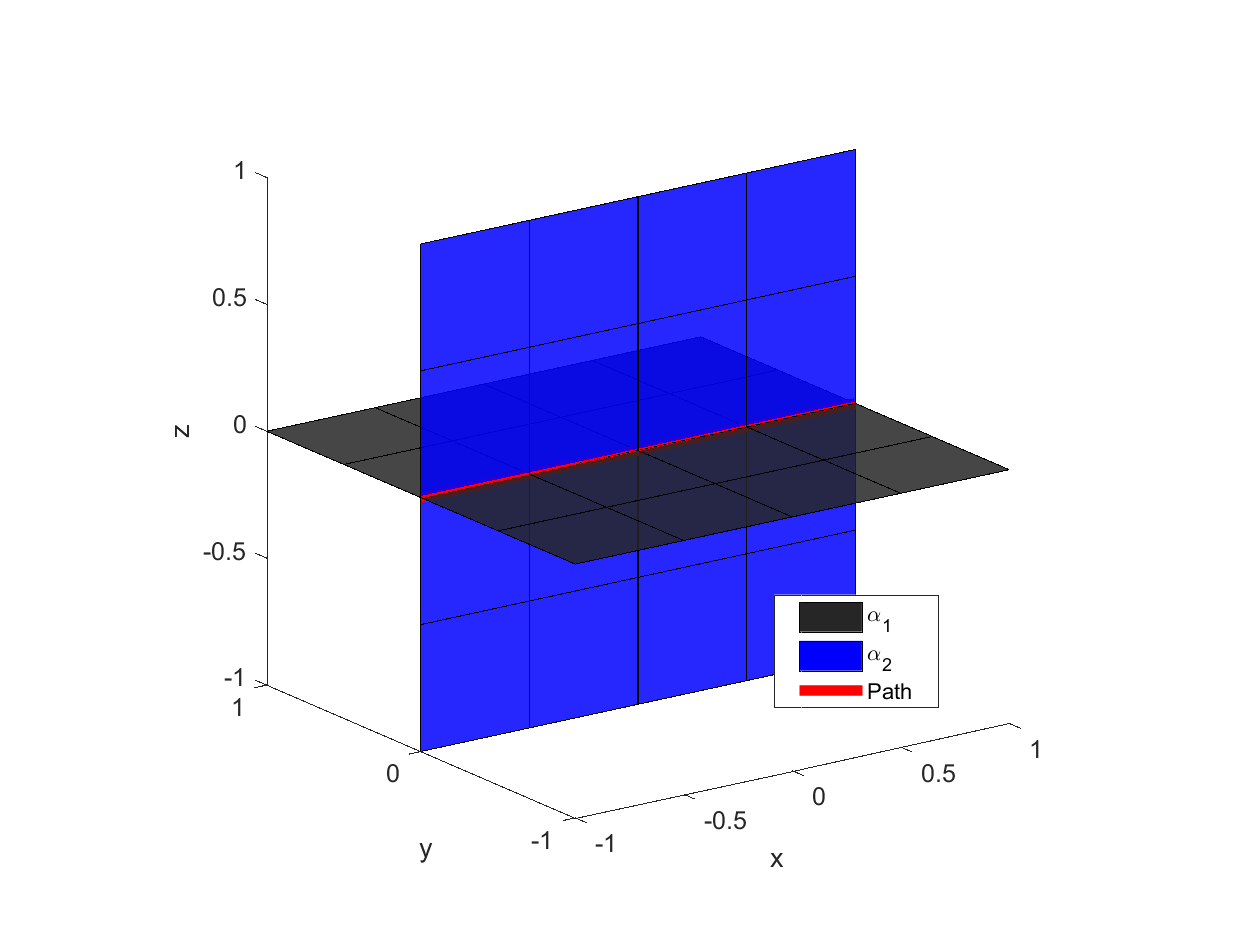
\includegraphics[trim=0 20 0 20,clip,width=10cm]{Figures/newIntersection}
	\caption{Plane intersection}
	\label{fig:planeIntersection}
\end{figure}

The significance of the circulation weight $H$ is that it allows for modification of the guidance behavior, i.e how abrupt the transition is between path convergence and circulation, without the need to re-derive the vector field equations. Guidance for a UAV heading at angle $\delta = 0$, representing a straight path in the x-direction, and equal parts circulation and convergence weights $G=H=1$ is shown in Figure \ref{fig:GVFLine}a. The potential function $V$ as shown in \cite{goncalves_artificial_2009,goncalves_circulation_2010,goncalves_vector_2010} decays to null at the target curve allowing circulation to dominate. Increasing the path following convergence $H$ increases this transition zone between convergence and path following, shown in Figure \ref{fig:GVFLine}b. 

\begin{figure}[H]
	\begin{subfigmatrix}{2}% number of columns
		\centering	
		\subfigure []{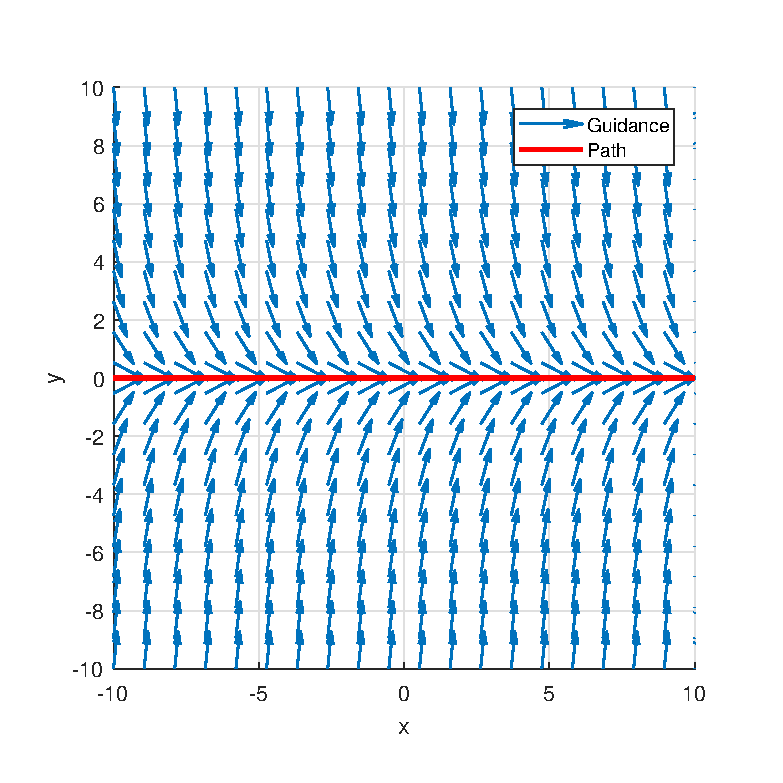
\includegraphics[trim=15 10 0 30,clip,width=8cm] {Figures/methods/straightPathH1}}
		\subfigure []{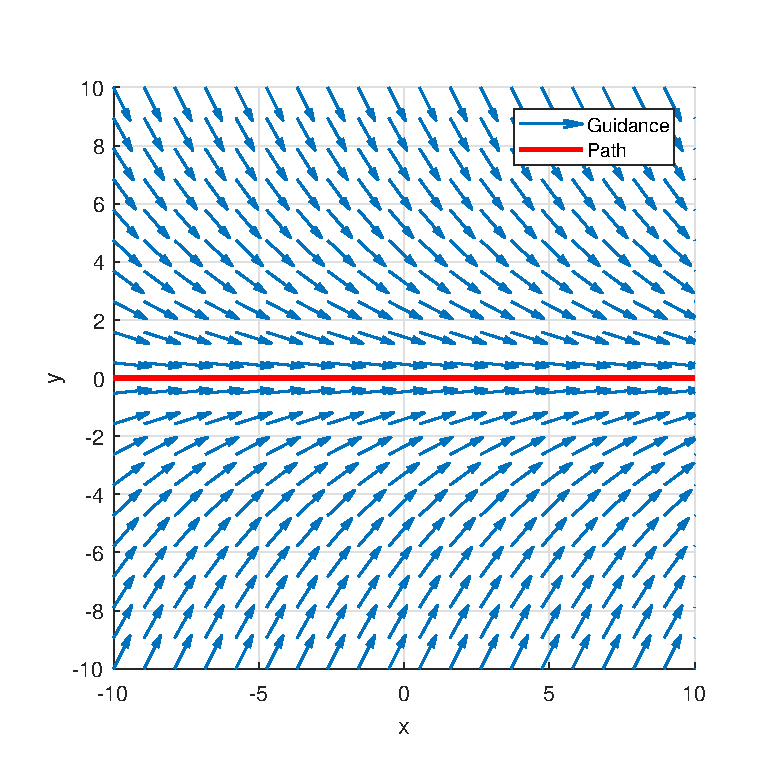
\includegraphics[trim=15 10 0 30,clip,width=8cm] {Figures/methods/straightPathH5}}
		
		\hspace*{0mm}
	\end{subfigmatrix}
	\caption{GVF converging and a) H=1 b) H=5}
	\label{fig:GVFLine}
\end{figure} 



\subsection{Avoidance}
Avoidance of circular areas with GVFs can be accomplished by negating the convergence weight $G$ and shrinking the path radius $r$, creating a repulsive field. Circular obstacles are considered. The circular avoidance vector field centered at $(x_c,y_c)$ and with radius $r$ is constructed by intersecting a cylinder, Equation \ref{eq:alphaCylinder}, and a plane Equation \ref{eq:pathFunctionZ}. 

\begin{equation}\label{eq:alphaCylinder}
\alpha_1 = (x-x_c)^2 + (y-y_c)^2-r^2
\end{equation}


Convergence can be calculated by the gradient of a potential function in Equation \ref{eq:potentialFunctionGrad}, which evaluates to

\begin{equation}
\nabla V = \dfrac{-1}{\sqrt{\bar{x}^4+\bar{y}^4+2\bar{x}^2\bar{y}^2-2r^2\bar{x}^2-2r^2\bar{y}^2+r^2+z^2}}\begin{bmatrix} 2\bar{x}^3+2\bar{x}\bar{y}^2-2r^2\bar{x} \\ 2\bar{y}^3+2\bar{x}^2\bar{y}-2r^2\bar{y} \\z \end{bmatrix}
\end{equation}

where


\begin{equation}
\bar{x} = x - x_c
\end{equation}
\begin{equation}
\bar{y} = y - y_c
\end{equation}

Circulation is calculated from the cross product of each implicit surface function's gradient, which equates to

\begin{equation}\label{eq:vcirc_circle}
\overrightarrow{V}_{circ} =  \begin{bmatrix}  2(y-y_c) \\[6pt] -2(x-x_c) \\[6pt] 0\end{bmatrix}
\end{equation}



Strictly repulsion guidance for a circular obstacle can be produced by assigning a negative weight to the convergence term $G=-1$, no circulation $H=0$, and a small path radius $r$. Reducing the radius $r$ helps to prevent the UAV  from entering a region of guidance that directs it towards a singular point, called a trap situation. Limiting the distance at which the field has influence is achieved with a decay function shown in Equation \ref{eq:decay} where $d$ is the range to the center of the obstacle and $R$ is the radius where the field has near zero strength. 

\begin{equation}
\label{eq:decay}
P = -\tanh \bigg( \frac{2\pi d}{R}-\pi\bigg)+1
\end{equation}

\begin{equation}
\label{eq:range}
d = \sqrt{ \bar{x}^2+\bar{y}^2}
\end{equation}

A strictly repulsive field $\overrightarrow{V}_{obst}$ with $G=-1$, $H=0$, $r=0.01$, and $R = 35$ is shown in Figure \ref{fig:decayApplied}a. Adding equal magnitude circulation and decay $G=-1$, $H=1$ is shown in Figure \ref{fig:decayApplied}b to demonstrate the effects of circulation on an avoidance field.


% ====== KEEP FOR THESIS =========
%Guidance for avoiding a circular path with a large radius can be produced by setting the convergence weight $G=-1$ and circulation weight $H=0$, shown in Figure \ref{fig:largerepulsive}. 
%
%\begin{figure}[H]
%	\centering
%	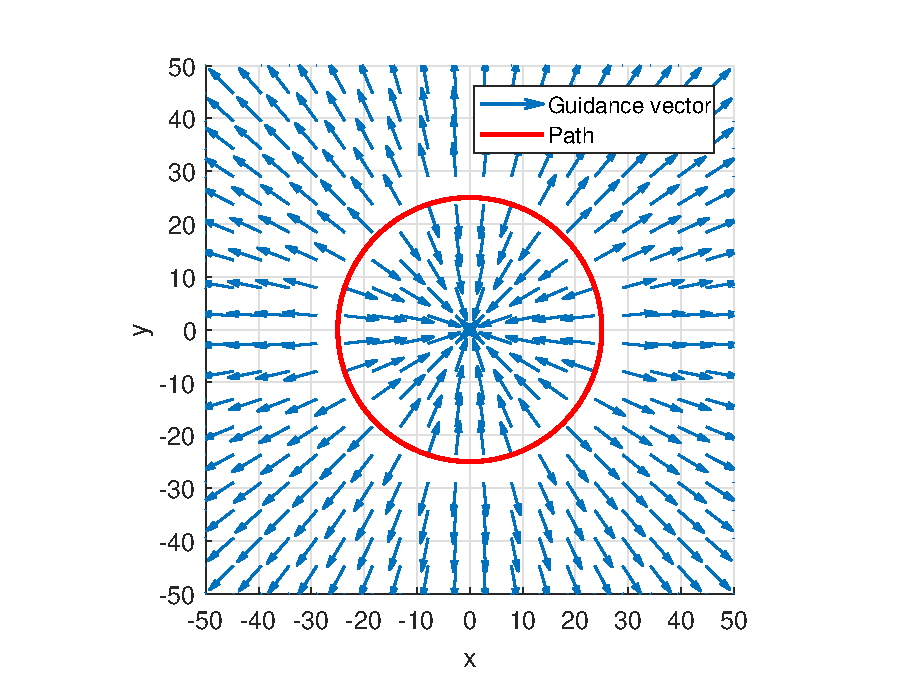
\includegraphics[width=0.7\linewidth]{Figures/methods/largeRepulsive}
%	\caption{Repulsive Circular Field with Large Radius}
%	\label{fig:largerepulsive}
%\end{figure}
%
%Note that inside of the path, vectors point towards the center of the circle which may produce a trap situation if the UAV ends up inside the radius. The radius of the path can be reduced, as shown in Figure \ref{fig:normalizedrepulsive} where $r=0.01$, to prevent trap situations.
%
%
%\begin{figure}[H]
%	\centering
%	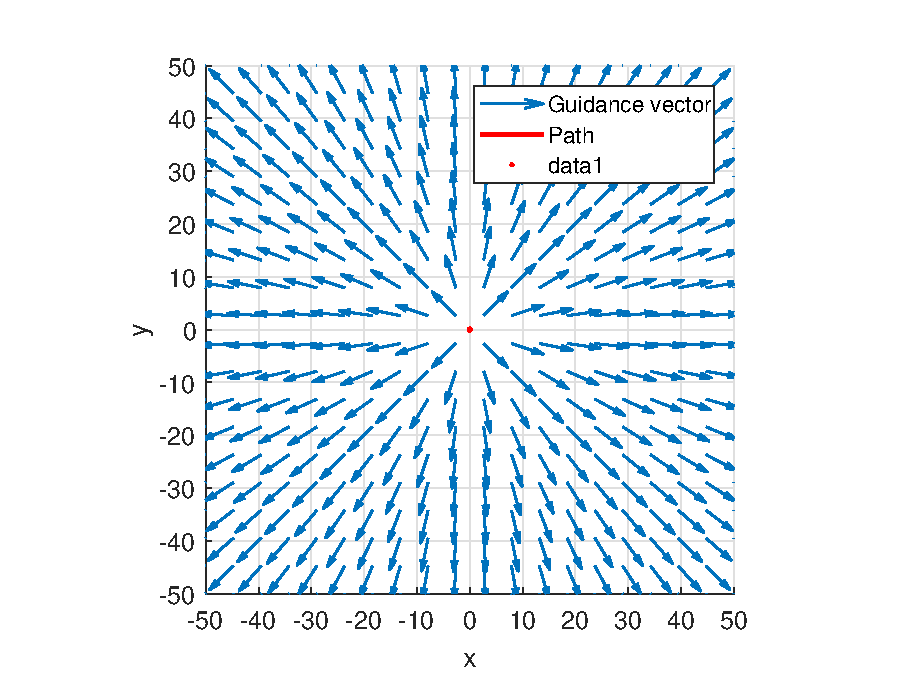
\includegraphics[width=0.7\linewidth]{Figures/methods/normalizedRepulsive}
%	\caption{Repulsive Circular Field with Small Radius}
%	\label{fig:normalizedrepulsive}
%\end{figure}
%
%Obstacle fields should only act locally on a UAV guidance which is accomplished by applying a decay function for a field of radius $R$. The decay strength $P$ is determined in \ref{eq:decay}, where $d$ is the euclidean distance, or range, between the UAV and the center of the obstacle, shown in Equation \ref{eq:range}. At a distance $d>R$ the decay strength $P$ is effectively zero, having virtual no influence on the total guidance. At a distance $d\leq R$, the field strength is bounded between $[0,2]$.
%
%
%
%
%Applying the decay function with a decay edge radius $R = 35$ to the GVF shown in figure \ref{fig:normalizedrepulsive}, results in the field shown in Figure \ref{fig:decayapplied}.
%

%\begin{figure}[H]
%	\centering
%	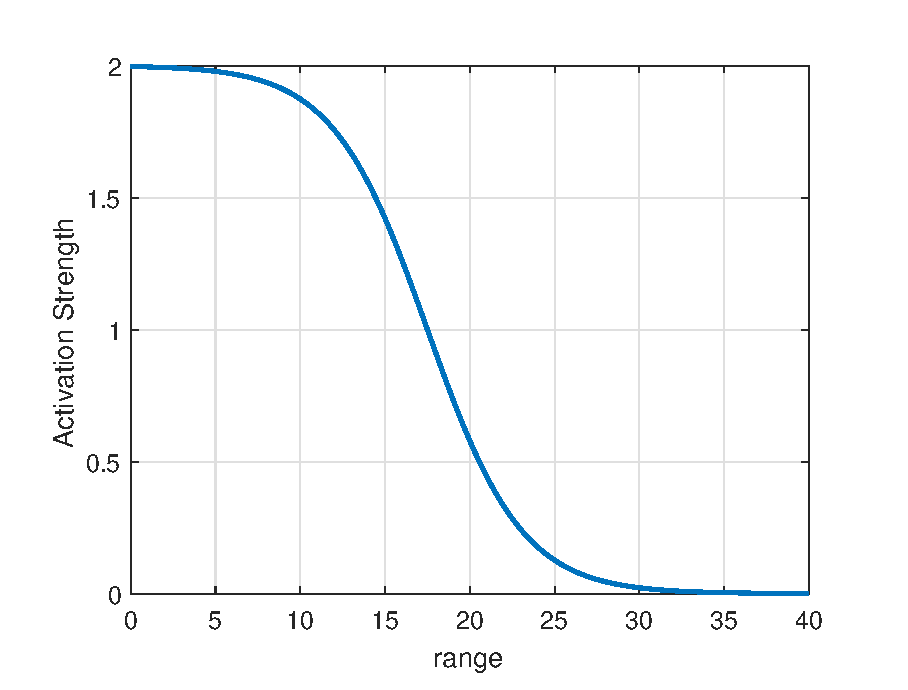
\includegraphics[width=0.7\linewidth]{Figures/methods/tanH}
%	\caption{}
%	\label{fig:tanh}
%\end{figure}


\begin{figure}[H]
	\begin{subfigmatrix}{2}% number of columns
		\centering	
		\subfigure []{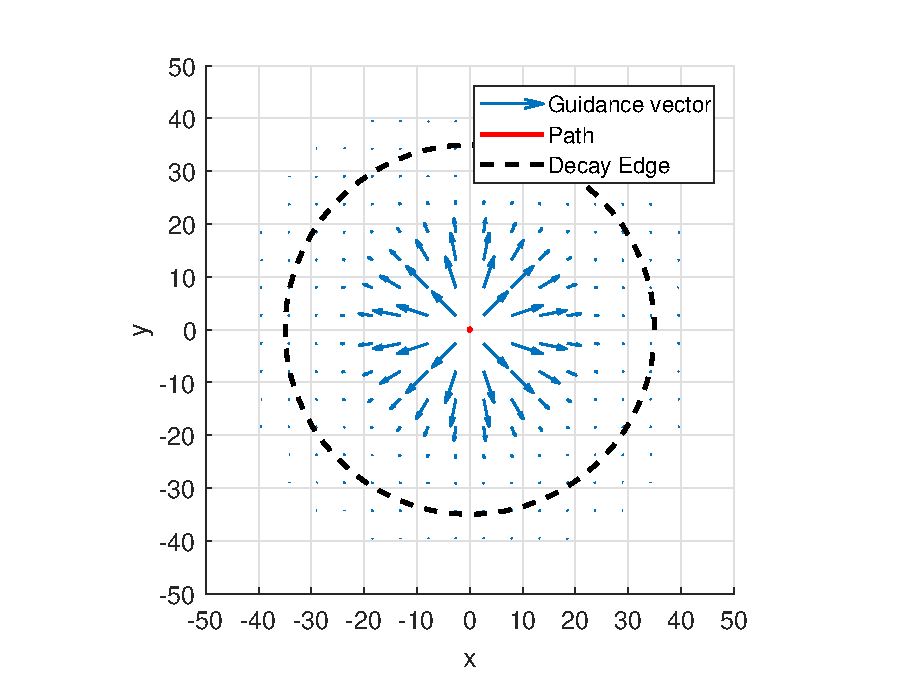
\includegraphics[trim=0 10 20 20,clip,width=8cm] {Figures/methods/decayApplied}}
		\subfigure []{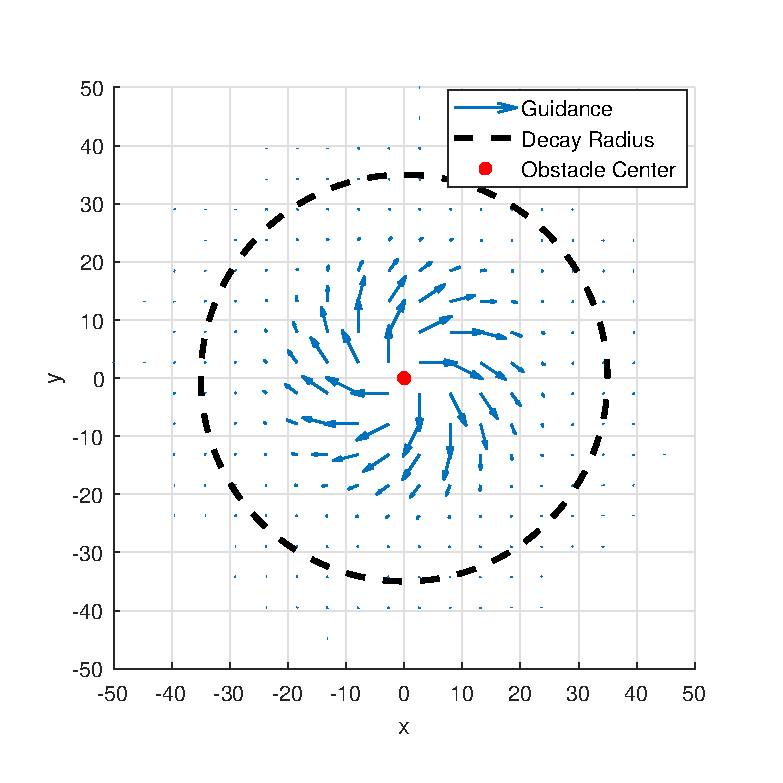
\includegraphics[trim=0 10 20 20,clip,width=8cm] {Figures/methods/decayAppliedCirculation}}
		\hspace*{0mm}
	\end{subfigmatrix}
	\caption{Repulsive GVF a) no circulation and b) with circulation}
	\label{fig:decayApplied}
\end{figure} 




%\begin{figure}[H]
%	\centering
%	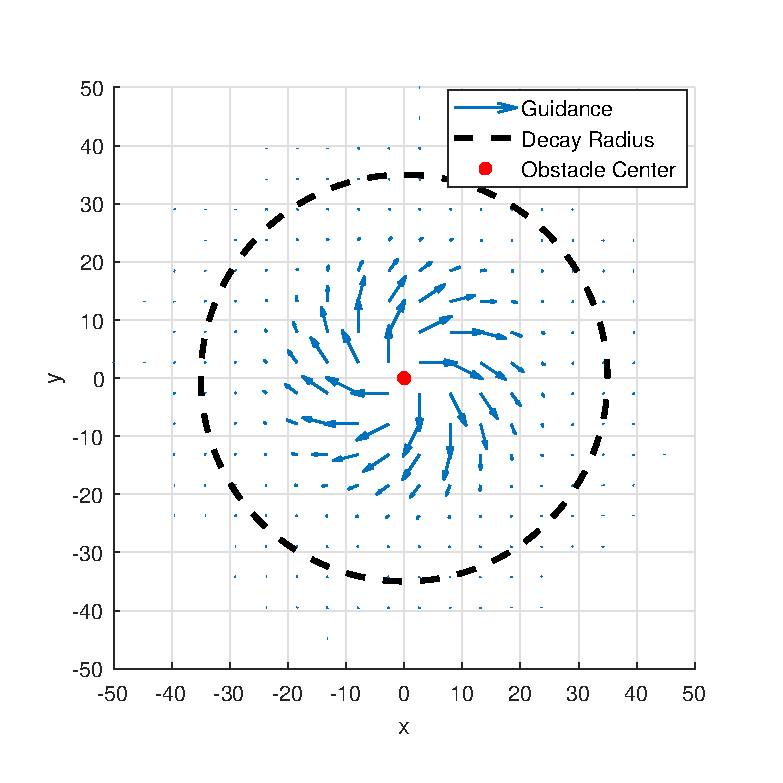
\includegraphics[width=0.7\linewidth]{Figures/methods/decayAppliedCirculation}
%	\caption{}
%	\label{fig:decayappliedcirculation}
%\end{figure}

Path following guidance and repulsive obstacle avoidance is achieved by summing the two fields together, shown in Equation \ref{eq:totalGuidanceObstacleLit}.




\subsection{Singularity Detection}
Summing vector field guidance may result in singularities, regions regions where vectors directly and equally oppose each other resulting in a null guidance. Singularities may be problematic if the UAV passes directly through one, which may result in trap situations or failure to avoid an obstacle. Singularities may exist where the magnitude of the vector $\overrightarrow{V}_g$ has a magnitude equal to zero, shown in Equation \ref{eq:singularityCondition}. Analytical solutions to singularity condition may be difficult to obtain when the path is non-linear and multiple solutions may also exist. A numerical search with initial conditions placed at the radius of equal strength, $R/2$, can be used to determine the location of singularities in the summed GVF guidance. 


 \begin{equation}
\label{eq:singularityCondition}
||\overrightarrow{V}_g || = 0
\end{equation}

A worst case scenario for singularities occurs when a strictly repulsive GVF is centered on a path. Vectors from both path following and obstacle fields directly oppose each other, leading to vector cancellation on the radius of equal strength. Singularities are detected in the described situation by searching for null magnitude vectors, shown in Figure \ref{fig:singularity-example}. 

\begin{figure}[H]
	\centering
	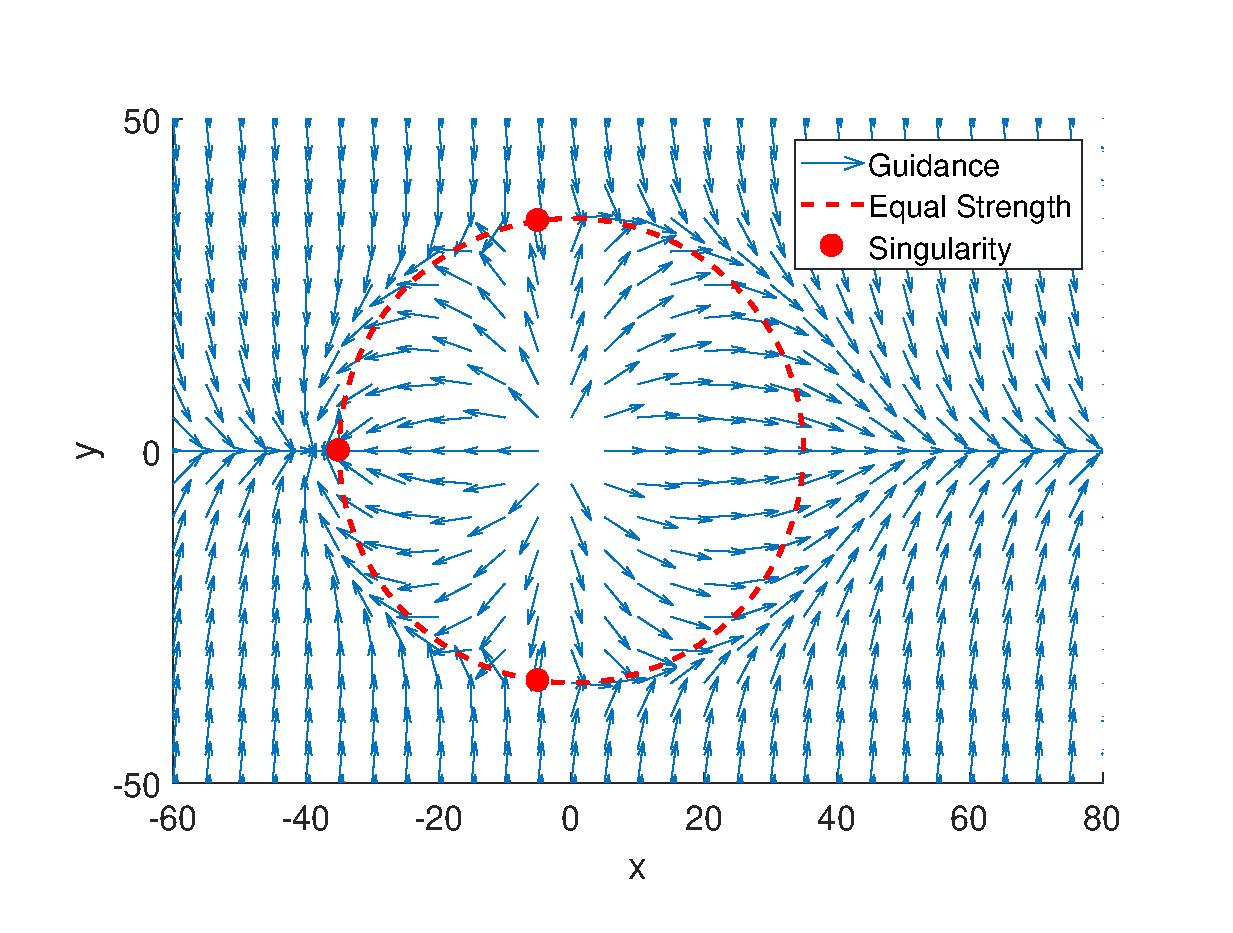
\includegraphics[trim=0 10 0 30, clip,width=12cm]{Figures/methods/singularityexample}
	\caption{Summed guidance and GVF singularities for strictly repulsive obstacle field}
	\label{fig:singularity-example}
\end{figure}

In order to modify the location of vector field singularities the behavior of either the path following or repulsive field needs to be modified. Increasing the path following field's circulation so the vectors are more parallel to the target path could eliminate the singularities at the 12 o'clock and 6 o'clock position of the obstacle, however would not effect the left most singularity. Additionally, increasing circulation would increase the time taken for he UAV to converge to the target path. Modifying the circulation of the obstacle, however, accomplishes two things. First, it provides information on how to circumnavigate the obstacle. Second, circulation would crate a perpendicular component to the obstacle vectors that may aid in preventing singularities from forming. Determining what circulation weight $H$ is necessary for avoiding a circular obstacle was accomplished by minimizing a path deviation cost function.



 
%Multiple singularities or near zero guidance regions may exist, so several initial conditions must be evaluated to increase the probability of detection. With the path and obstacle field shown in \ref{fig:summedquiver}, several initial conditions evenly spaced were evaluated both inside and outside of the equal strength circle. Note how only points left of the obstacle were evaluated since this region is where attractive and repulsive vectors oppose each other, therefore it is where singularities are expected. Both inside and outside initial conditions determine the location of the singularities. 




%Solving for the location of singularities using a numerical solver with initial conditions placed at the radius of equal strength for the field in \ref{fig:summedquiver} is shown in Figure \ref{fig:noCircSingularityDetection}a. Modifying the repulsive field with a non-zero circulation weight can reduce the number of singularities as well as remove them for the UAVs path. Additionally, circulation directs the UAV around obstacle in a deterministic way. A circulation weight of $H=1$ produces the guidance with a singularity removed from the path shown in Figure \ref{fig:noCircSingularityDetection}b. Determining the exact values of $R$ and $H$ to produce an avoidance guidance that minimizes deviation from the path will now be discussed. 




%\begin{figure}
%	\centering
%	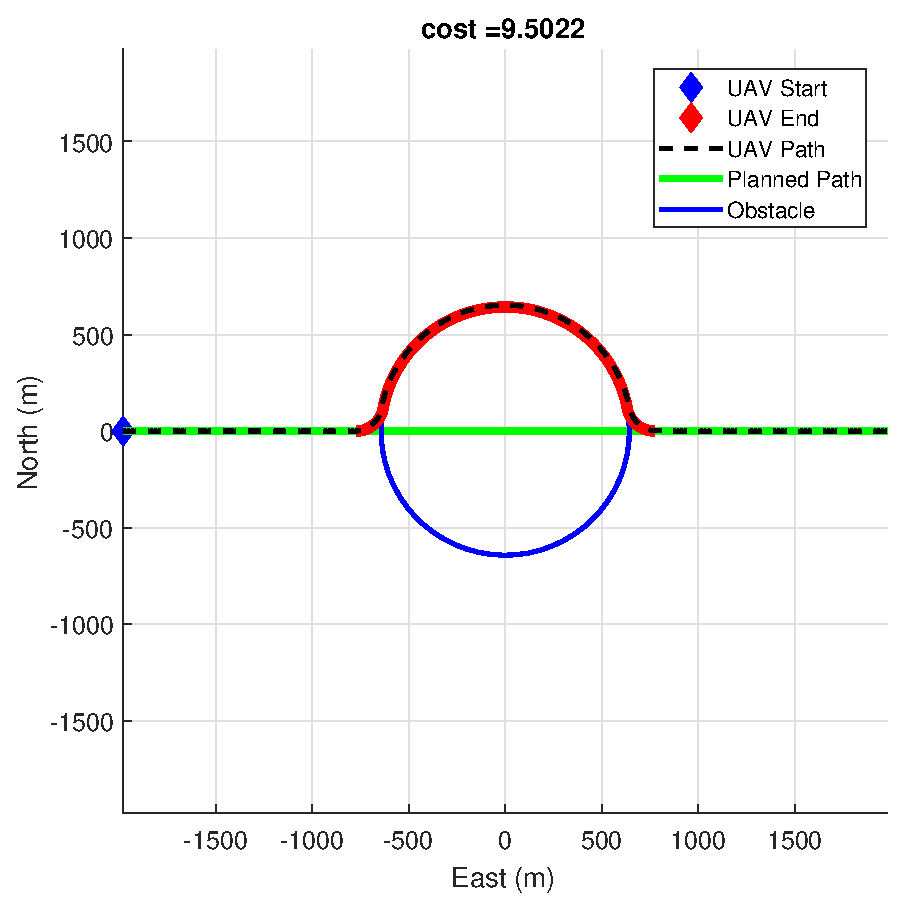
\includegraphics[width=0.7\linewidth]{Figures/semiFinalAlgorithm/Obsty0}
%	\caption{}
%	\label{fig:obsty0}
%\end{figure}
%\begin{figure}
%	\centering
%	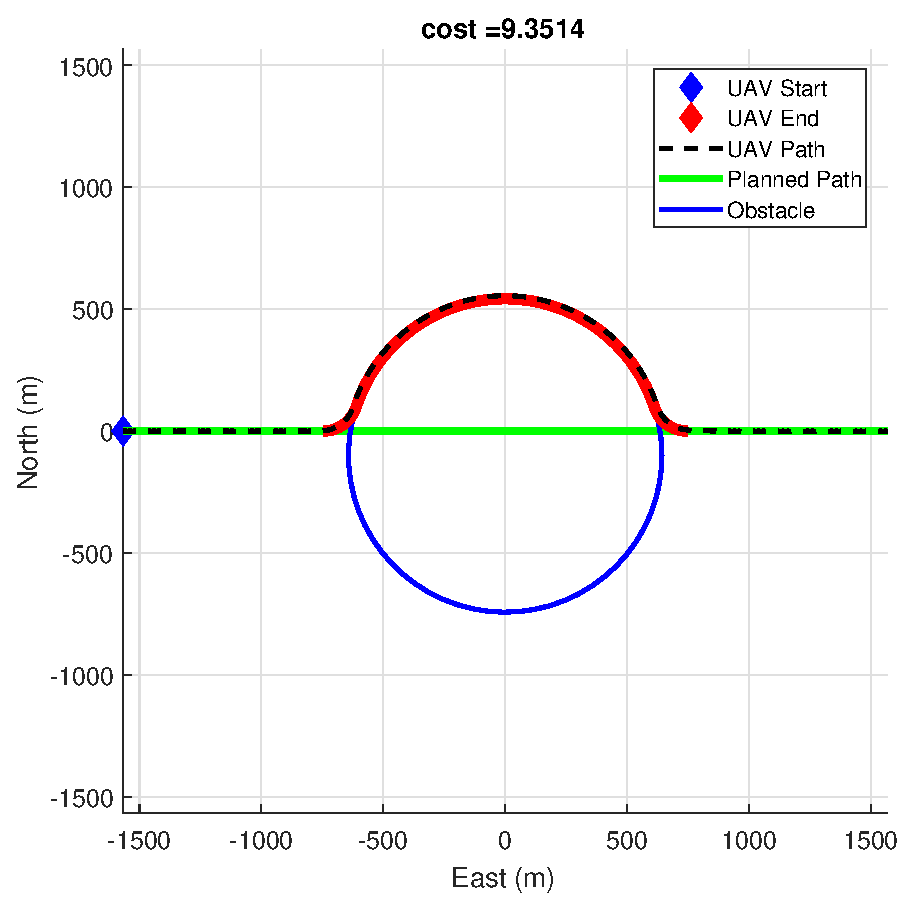
\includegraphics[width=0.7\linewidth]{Figures/semiFinalAlgorithm/Obsty-100}
%	\caption{}
%	\label{fig:obsty0}
%\end{figure}
%
%\begin{figure}
%	\centering
%	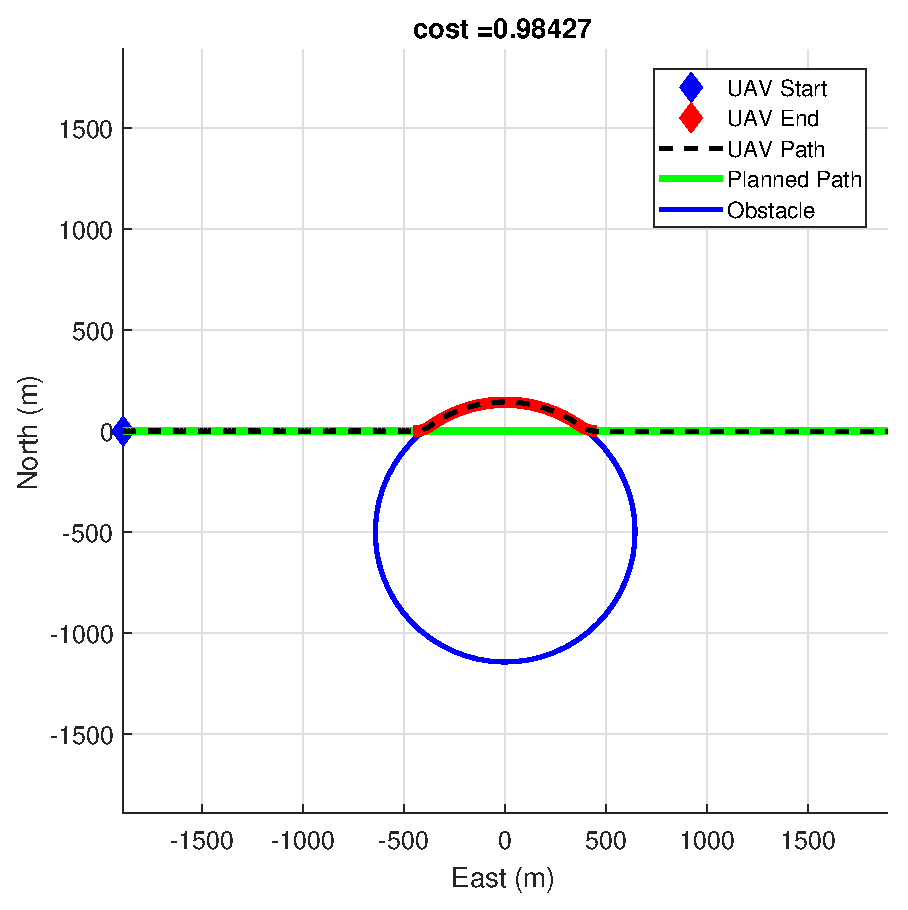
\includegraphics[width=0.7\linewidth]{Figures/semiFinalAlgorithm/Obsty-500}
%	\caption{}
%	\label{fig:obsty0}
%\end{figure}
%
%
%\begin{figure}
%	\centering
%	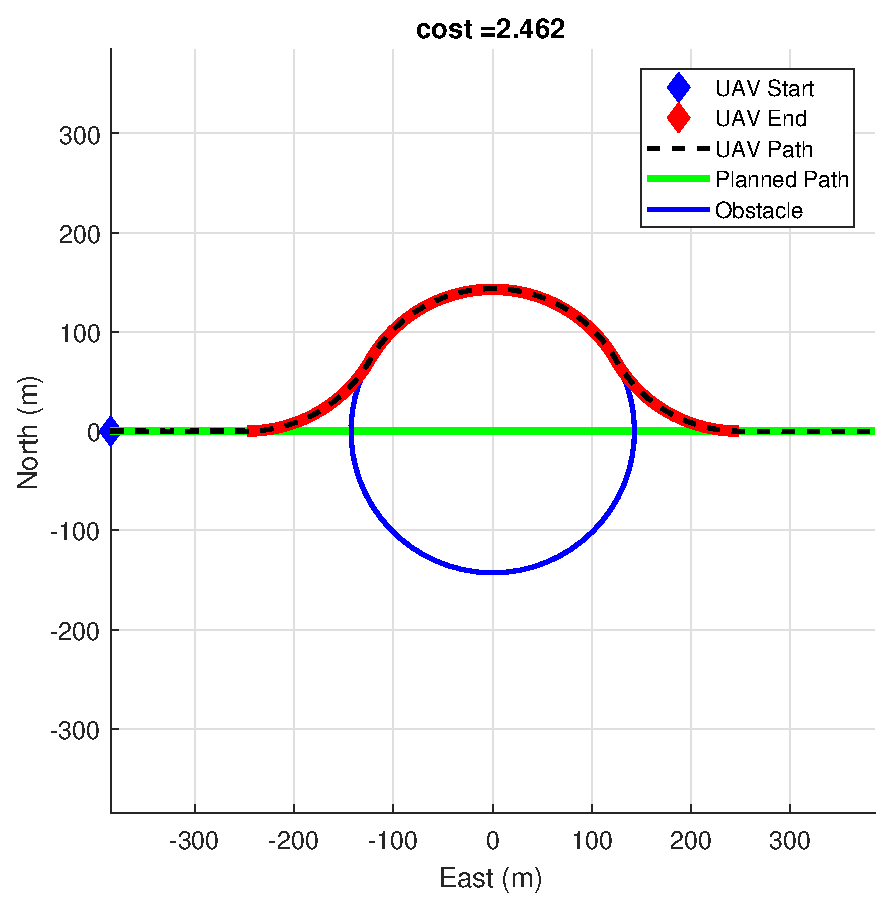
\includegraphics[width=0.7\linewidth]{Figures/semiFinalAlgorithm/ObstR142}
%	\caption{}
%	\label{fig:obsty0}
%\end{figure}
%
%\begin{figure}
%	\centering
%	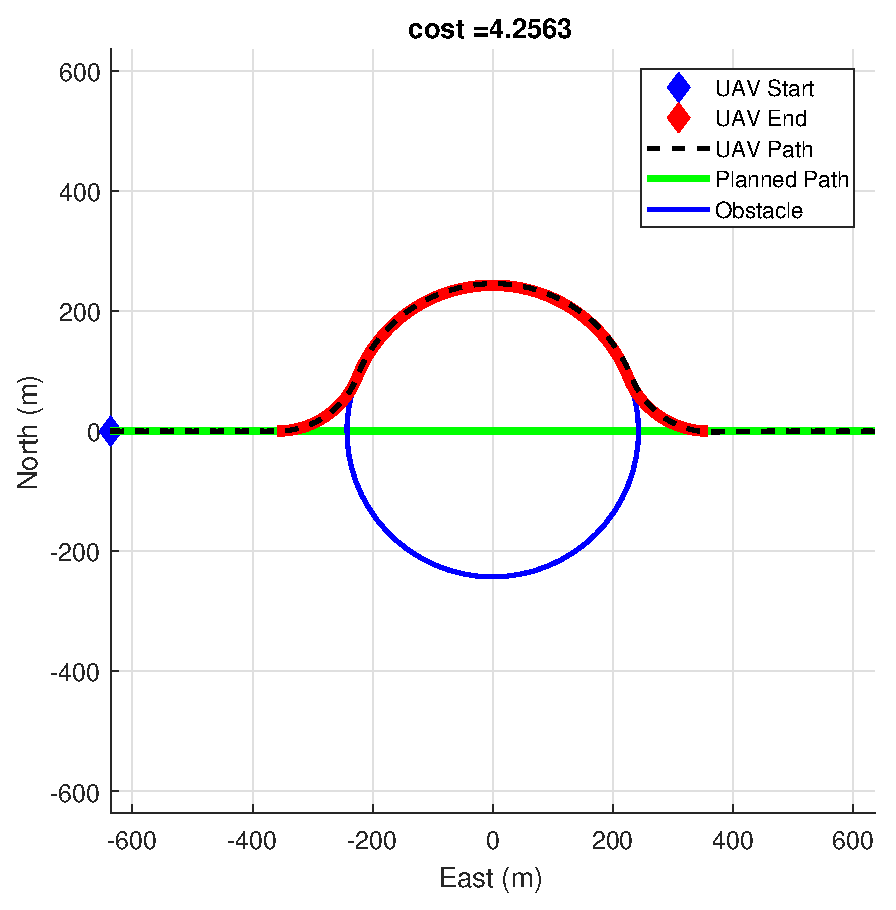
\includegraphics[width=0.7\linewidth]{Figures/semiFinalAlgorithm/ObstR242}
%	\caption{}
%	\label{fig:obsty0}
%\end{figure}
%
%\begin{figure}
%	\centering
%	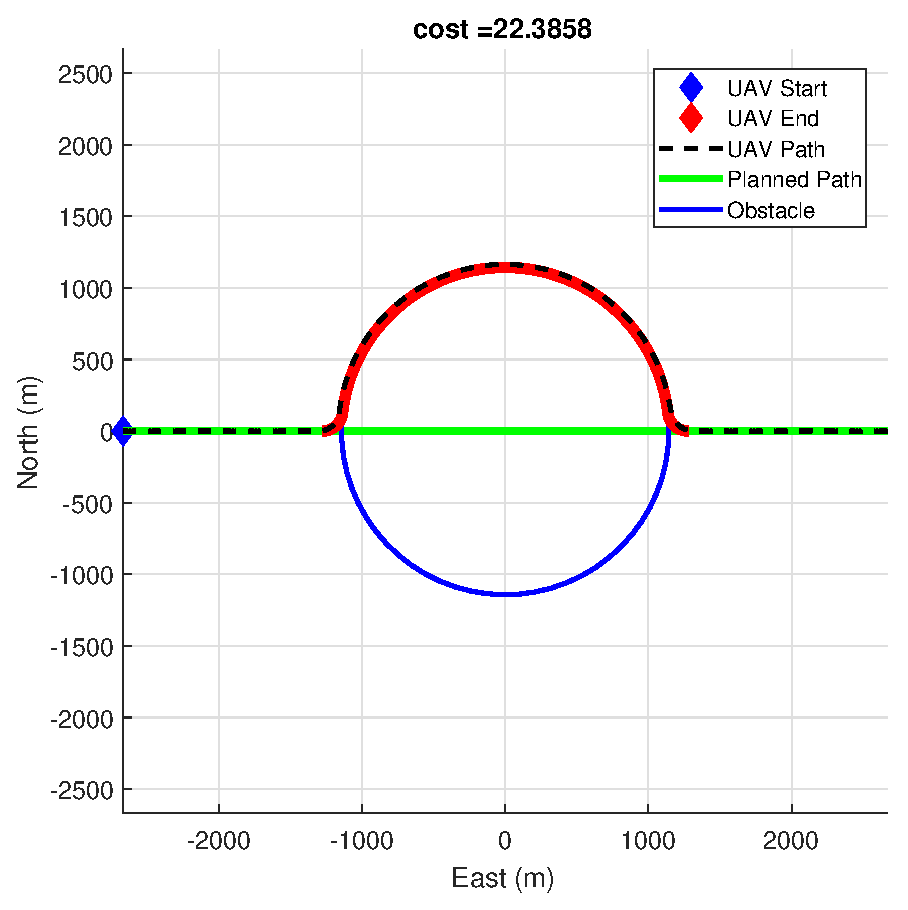
\includegraphics[width=0.7\linewidth]{Figures/semiFinalAlgorithm/ObstR1142}
%	\caption{}
%	\label{fig:obsty0}
%\end{figure}
%
%\begin{figure}
%	\centering
%	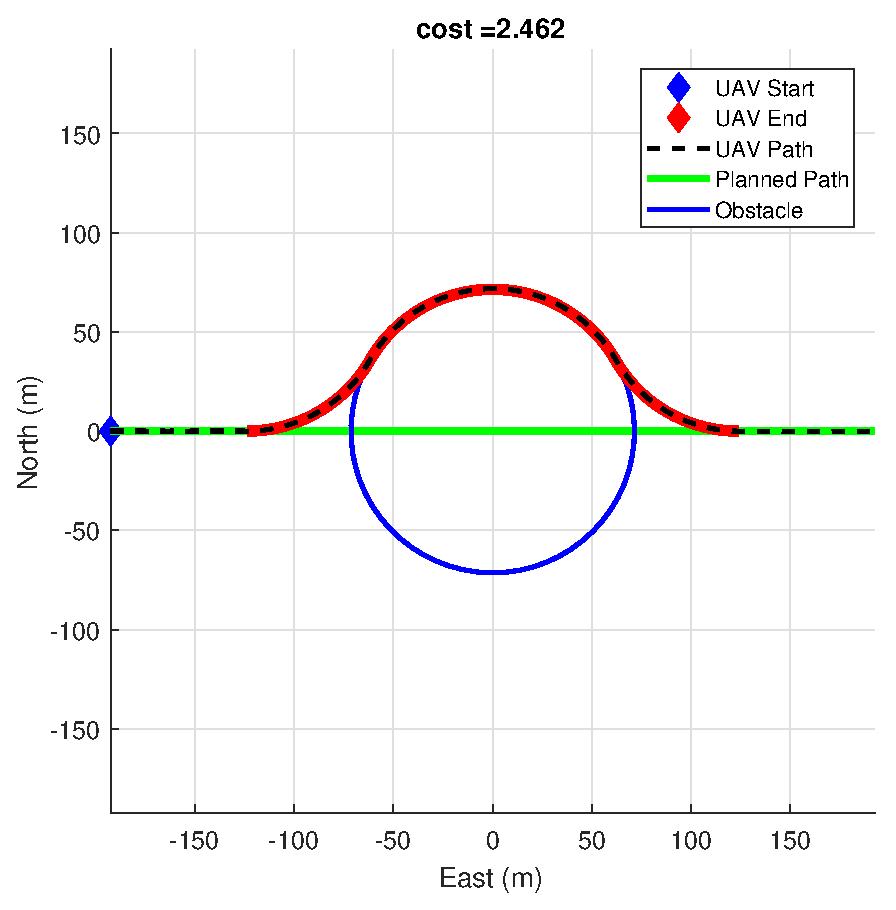
\includegraphics[width=0.7\linewidth]{Figures/semiFinalAlgorithm/Vs25}
%	\caption{}
%	\label{fig:obsty0}
%\end{figure}
%
%\begin{figure}
%	\centering
%	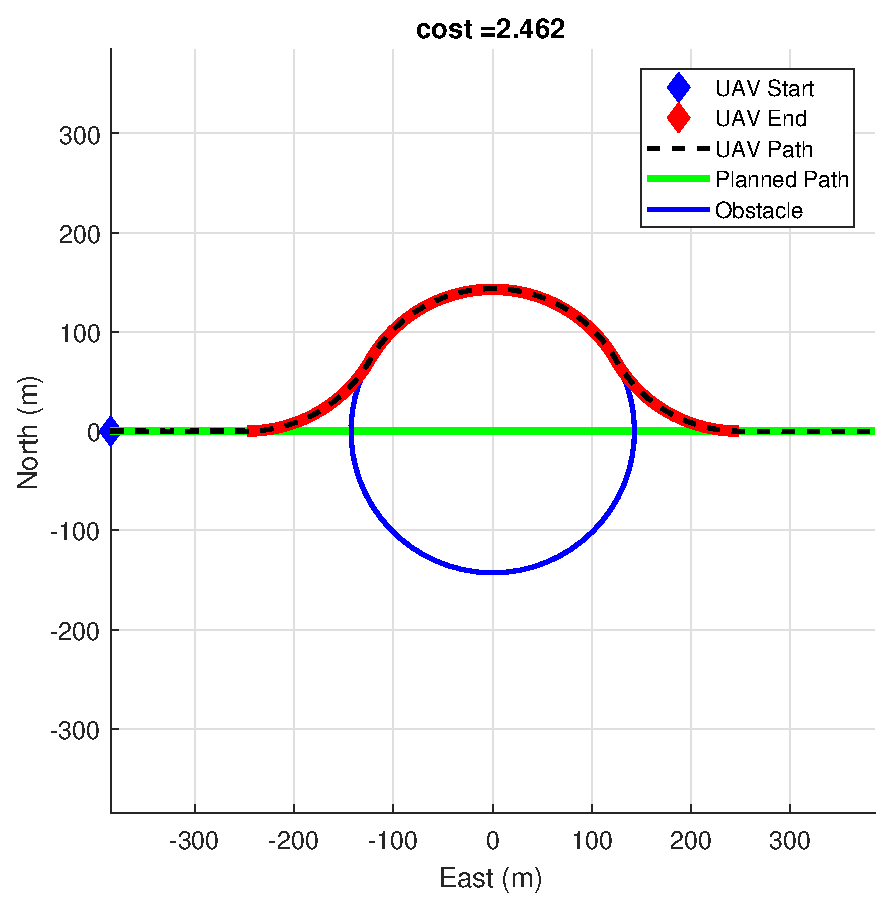
\includegraphics[width=0.7\linewidth]{Figures/semiFinalAlgorithm/Vs50}
%	\caption{}
%	\label{fig:obsty0}
%\end{figure}
%
%\begin{figure}
%	\centering
%	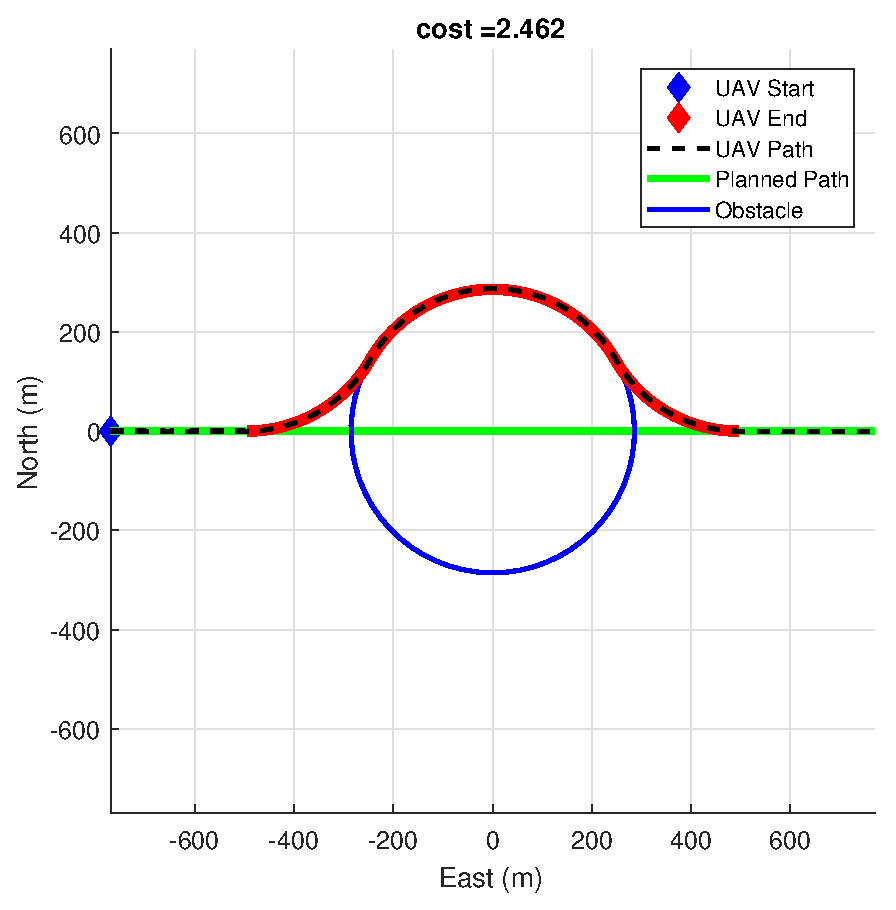
\includegraphics[width=0.7\linewidth]{Figures/semiFinalAlgorithm/Vs100}
%	\caption{}
%	\label{fig:obsty0}
%\end{figure}



%\subsection{Flight Envelope}
%Evaluating a large number of initial conditions to improve the probability of finding singularities may be computationally expensive and may also find singularities the UAV may not encounter. Selecting a reduced set of initial conditions and to determine if the singularities exist where the UAV may fly, a flight envelope is determined for some time horizon $t_h$. Consider the UAV depicted in Figure \ref{fig:flightenvelope2} with a turn rate $\dot{\theta}$ and fixed speed $u$. 
%
%\begin{figure}[H]
%	\centering
%	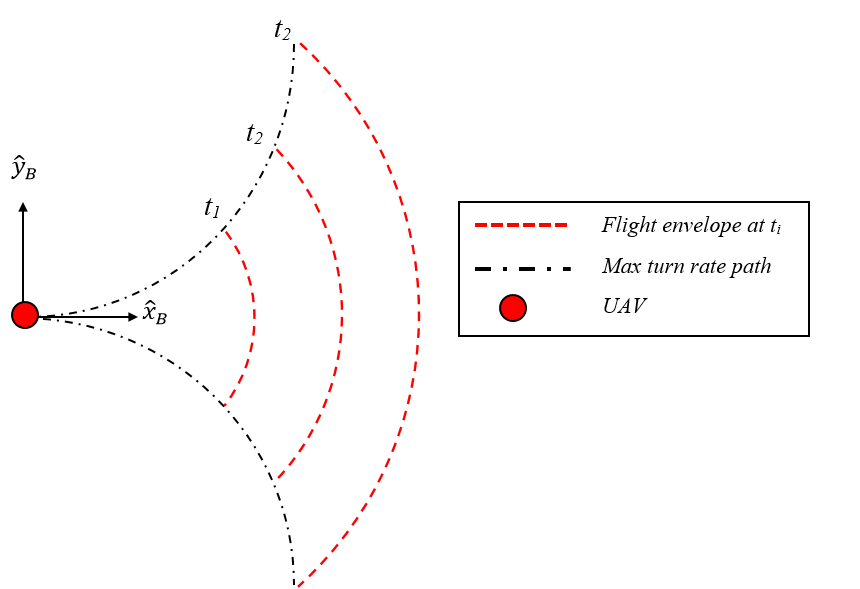
\includegraphics[width=0.7\linewidth]{Figures/methods/flightEnvelope2}
%	\caption{}
%	\label{fig:flightenvelope2}
%\end{figure}
%
%The flight envelope, or positions the UAV, at time $t_i$ with respect to the body frame is calculated in Equations \ref{eq:qx} and \ref{eq:qy}
%
%\begin{equation}
%\label{eq:qx}
%q_x =  \frac{u}{\dot{\theta}} \sin(t_h \dot{\theta})
%\end{equation}
%
%\begin{equation}
%\label{eq:qy}
%q_y =  \frac{u}{\dot{\theta}} \big(1-\cos(t_h \dot{\theta})\big)
%\end{equation}
%
%It is convenient to represent points on the flight envelope in the global inertial frame. The flight envelope points $(q_x,q_y)$ can be expressed in vector form by finding the angle $\phi$ with respect to the body frame $\hat{x}_b$ axis and the vector magnitude $q$ shown in equations \ref{eq:qphi} and \ref{eq:qMag} respectively.
%
%
%
%\begin{equation}
%\label{eq:qphi}
%\phi = \tan^{-1} \bigg( \frac{q_y}{q_x} \bigg)
%\end{equation}
%
%\begin{equation}
%\label{eq:qMag}
%q = \sqrt{q_x^2 +q_y^2}
%\end{equation}
%
%
%
%\begin{equation}
%\label{eq:pos}
%\overrightarrow{Q_b} = \begin{bmatrix}
%	q\cos\phi \\
%	q\sin\phi \\
%	0
%\end{bmatrix}
%\end{equation}
%
%To express the flight envelope in the global inertial frame, the position vector of the UAV $\overrightarrow{P}_0$ and $\theta$ are applied with a rotation matrix $R$, shown in Equations \ref{eq:pos}, \ref{eq:rotation}, and \ref{eq:qGlobal} below. 
%
%
%\begin{figure}[H]
%	\centering
%	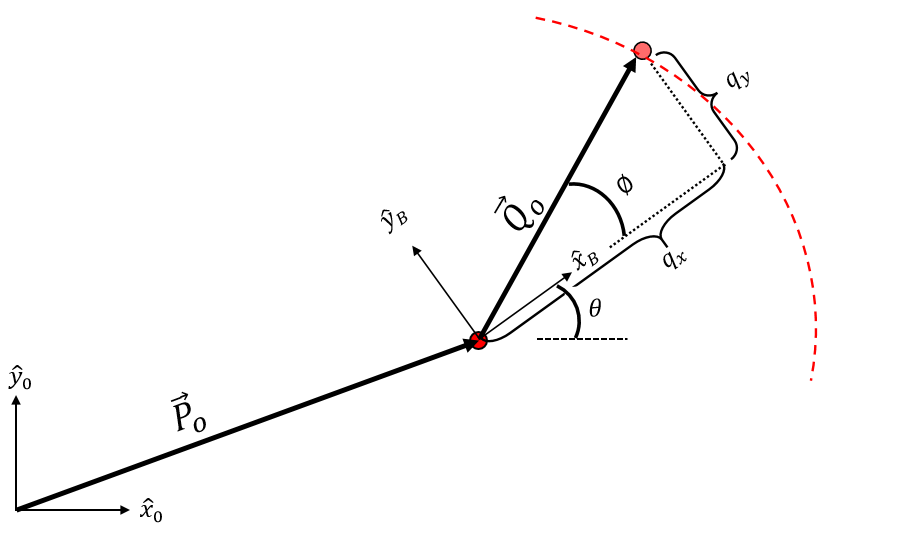
\includegraphics[width=0.7\linewidth]{Figures/methods/flightEnvelope}
%	\caption{}
%	\label{fig:flightenvelope}
%\end{figure}
%
%
%\begin{equation}
%\label{eq:rotation}
%\overrightarrow{P}_0 = \begin{bmatrix}
%x & y & 0
%\end{bmatrix}^T
%\end{equation}
%
%
%\begin{equation}
%\label{eq:qGlobal}
%   R=\begin{bmatrix}
%	\cos(\theta) & -\sin(\theta) & 0 \\
%	\sin(\theta) & \cos(\theta) & 0 \\
%	0 & 0 & 1 \\
%\end{bmatrix}
%\end{equation}
%
%
%\begin{equation}
%\label{eq:pos}
%\overrightarrow{Q}_0 = \overrightarrow{P_0} + R  \overrightarrow{Q_b}
%\end{equation}
%
%Initial conditions placed on the flight envelope will follow the magnitude gradient of the GVF guidance and locate any singularities it may encounter. When a singularity is found to exist inside or near a flight envelope the field can be modified to counteract it. 



\subsection{Static Modified Weights}

Determining the decay radius $R$ and circulation weight $H$ for a repulsive vector field depends on the UAVs speed $u$ and turnrate $\dot{\theta}$. An obstacle located at a lateral distance $Y_0$ from the pre-planned sensor path has a radius $r_O$ equal to a scalar multiple of the UAVs turn radius, shown in Equation \ref{eq:m}. The multiple $m$ is bounded on the interval $[1,\infty)$.

\begin{equation}
\label{eq:m}
r_O = m \theta_r
\end{equation}

The repulsive field decay radius $R$, expressed in $k$ multiples of the obstacles radius is shown in Equation \ref{eq:k} and also bounded on the interval $[1,\infty)$.

\begin{equation}
\label{eq:k}
R = k r_O
\end{equation}

The decay multiple $k$ and circulation $H$ are then determined by minimizing the cost function $\ref{eq:staticCost}$, where $y$ is the lateral deviation from the path in the $I$ frame and the function $j$ penalizes the UAV for entering the obstacle radius. The sign of $H$ can be determined from the LOS angle between the UAV and the obstacle such that the UAV travels around the obstacle in the correct, least distance, direction.

\begin{equation}
\label{eq:staticCost}
\begin{aligned}
& \underset{H,k}{\text{minimize}}
& & \frac{1}{R}\int_{0}^{t_f}ydt + j(x,y) 
\end{aligned}
\end{equation}


\begin{equation}
j(x,y) = \left\{
\begin{array}{ll}
100dt & \quad \sqrt{(x-xc)^2+(y-yc)^2} \leq r_O \\
0 & \quad \sqrt{ (x-xc)^2+(y-yc)^2 } > r_O
\end{array}
\right.
\end{equation}




A comparison of a UAVs Dubins route using a strictly repulsive vector field versus a vector field with circulation is shown in Figure \ref{fig:noCircVsCirc}. A UAV with a speed of $u=20 m/s$ and turning rate of $\dot{\theta} = 20 deg/s$ following a straight vector field path is shown avoiding an obstacle of radius $m=1$. The optimized GVF shows a decrease in the path deviation function compared to the non-optimized GVF of $72 \% $.

\begin{figure}[H]
	\begin{subfigmatrix}{2}% number of columns
		\centering	
		\subfigure []{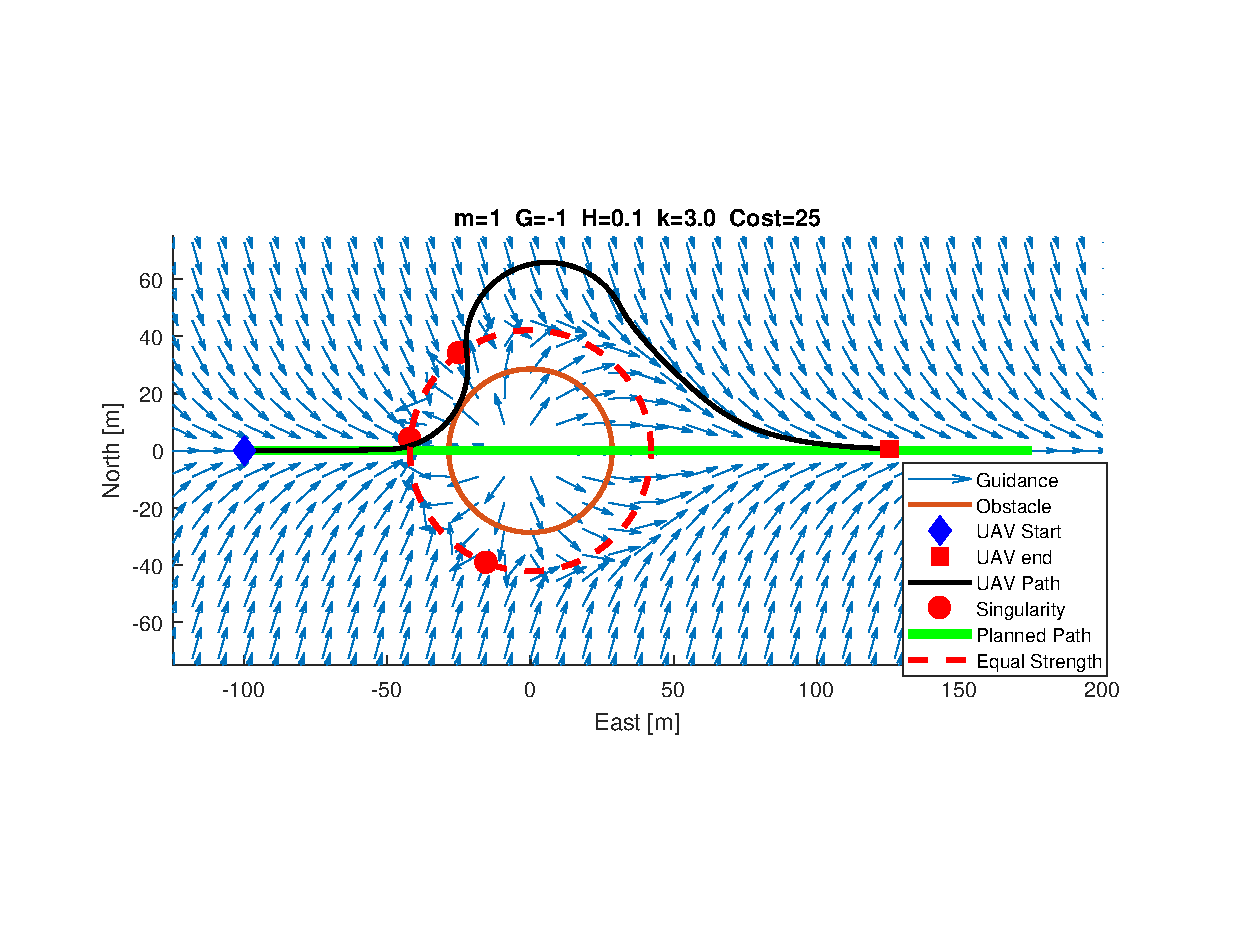
\includegraphics[trim=35 20 40 10,clip,width=7.5cm] {Figures/methods/bruteForceSolveN1V10}}
		\subfigure []{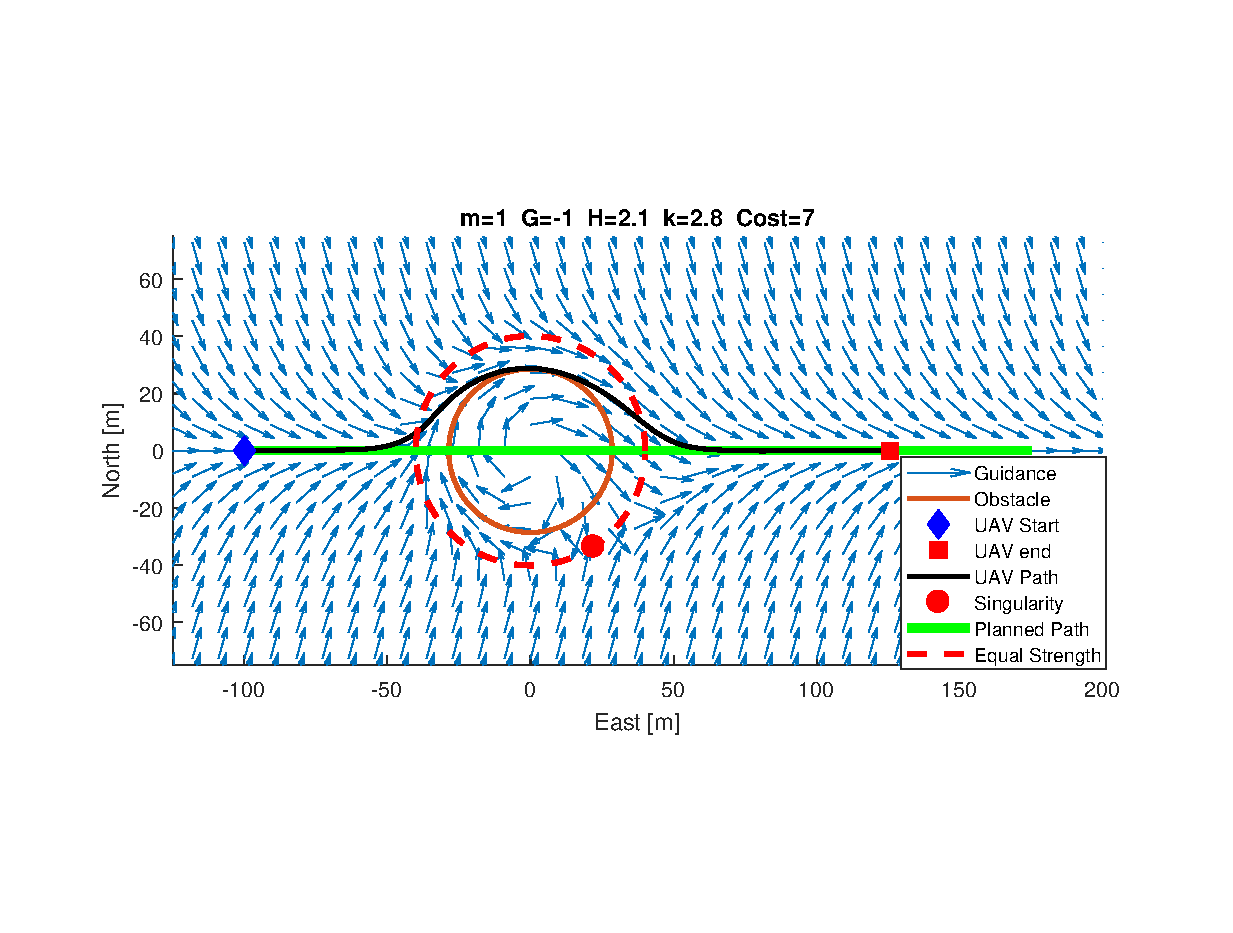
\includegraphics[trim=40 25 40 30,clip,width=7.5cm] {Figures/methods/solvedN1V10}}
		\hspace*{0mm}
	\end{subfigmatrix}
	\caption{Repulsive and Circulating VF Guidance UAV Route}
	\label{fig:noCircVsCirc}
\end{figure}





%\subsection{Modified Path Following Vector Field}
%The summed guidance results in the UAV leaving the path pre-maturely and slowly returns to the path. Gradually leaving and returning to the path is a result of the slow transition between attractive and repulsive field dominating the guidance. It is desired that the UAV follows the path up until the UAV must turn to avoid the obstacle and quickly return to the path. To accomplish this, a modification to attractive and repulsive fields must take place. Additionally, improved tracking of the outside of the obstacle can be achieved by modifying the convergence strength of the repulsive field. The modified vector field guidance with attractive weight $M$ and repulsive weight $N$ is considered without a decay function $P$, shown in Equation \ref{eq:modifiedGuidance}
%
%
%\begin{equation}
%\label{eq:modifiedGuidance}
%\overrightarrow{V}_g = M \overrightarrow{V}_{path} + N \overrightarrow{V}_{obst}
%\end{equation}
%
%
%While the UAVs horizontal position $x$ in the $I$ frame is less than the turning distance $\tilde{x}$, the attractive weight $M=1$ and the repulsive weight is null at $N=0$. Once the UAVs horizontal position reaches the turning distance, $x=\tilde{x}$ the attractive field weight switches to null $M=0$ and repulsive weight dominates at $N=1$. The repulsive field has a constant circulation of unity with sign equal to that of the UAVs lateral position with respect to the $I$ frame. Convergence becomes a function of the UAVs relative heading with respect to the obstacle center $\beta$, defined in Equation \ref{eq:beta}.  
%
%\begin{equation}
%\label{eq:beta}
%\beta = \pi - \tan^{-1} \Bigg(\frac{y-Y_0}{x}\Bigg) + \theta
%\end{equation}
%
%The convergence weight becomes:
%\begin{equation}
%\label{eq:gModified}
%g = -\cos(|\beta|)
%\end{equation}
%
%When the UAV has a heading towards the obstacle center, the repulsion is maximized at $-1$. As the UAVs heading becomes perpendicular to the LOS to the obstacle center, the repulsion falls off to zero and circulation dominates. If the UAVs heading begins to drift back towards the obstacle, either by wind or another external disturbance, $g$ will decrease to counteract the deviation. When the UAVs horizontal position $x>\hat{x}$ the repulsive field weight nulls $N=0$ and the attractive field becomes unity $M=1$. \\
%
%The modified VF guidance eliminates the need for a minimizer or lookup table, eliminates singularities since the two fields will never be equal strength, and provides a guidance comparable to waypoint guidance without the need to re-plan a path. 



\section{Simulations}

A worst case avoidance scenario was be used to compare the optimized GVF with waypoint, VFF, and the optimal path with respect to the path deviation cost function. A circular obstacle centered on the path, $y_o = 0$, requires a deviation from the path of at least $50\% $ of the obstacles radius. A fixed wing UAV at an initial position $(-400,0)$ and heading $\theta=0^\circ$ follows the straight path connecting the points $(-400,0)$ and $(400,0)$ respectively. Traveling at a constant speed $u=25 m/s$ and with a fixed turn rate of $\dot{\theta}=20 deg/s$ the UAV must avoid an obstacle with radius $2\theta_r$ located at the origin $(0,0)$. The VFF guidance from \cite{borenstein_real-time_1990} is used with an obstacle window radius of $\theta_r+r_o$, a cell repulsion $Fr=-3$, attraction force $F_t=0.8$, range exponent $n=2$, and a goal located at $(700,0)$. For LOS waypoint guidance, $7$ waypoints with a small waypoint radius of $10m$ was chosen. Each diversion waypoint added drives the guidance closer to optimal, however has diminishing returns past $6-7$ waypoints. GVF guidance with a circular repulsive field was assigned a convergence weight $G=-1$ and circulation and decay radius coefficient $k$ were determined by evaluating the cost function in Equation \ref{eq:staticCost} with initial conditions $k_i = 2$ and $H=2$. The GVF solution was bounded such that $2\leq k\leq 4$ and $1\leq H\leq 6$, determined from running a large range of simulations. Outside of the described bounds the UAV either failed to avoid the obstacle or entered a trap situation.  Minimizing the cost function, described in Equation \ref{eq:staticCost}, resulted in a decay radius coefficient $k=2.78$ and a circulation value $H=1.88$. The Dubin's paths for the three guidance methods discussed is shown in Figure \ref{fig:comparemethods}. \\

VFF results in a UAV route that has excess deviation from the planned path with excessive turns. Waypoint guidance returns to the path more quickly than VFF, however deviates from the planned path farther then necessary. GVF leaves the path before waypoint guidance and tracks the outside of the obstacle closely and then quickly converges back to the pre-planned path. The cost of each method, defined in Equation \ref{eq:staticCost}, is displayed in the bar plot shown in Figure \ref{fig:barplotperformance}.


\begin{figure}[H]
	\centering
	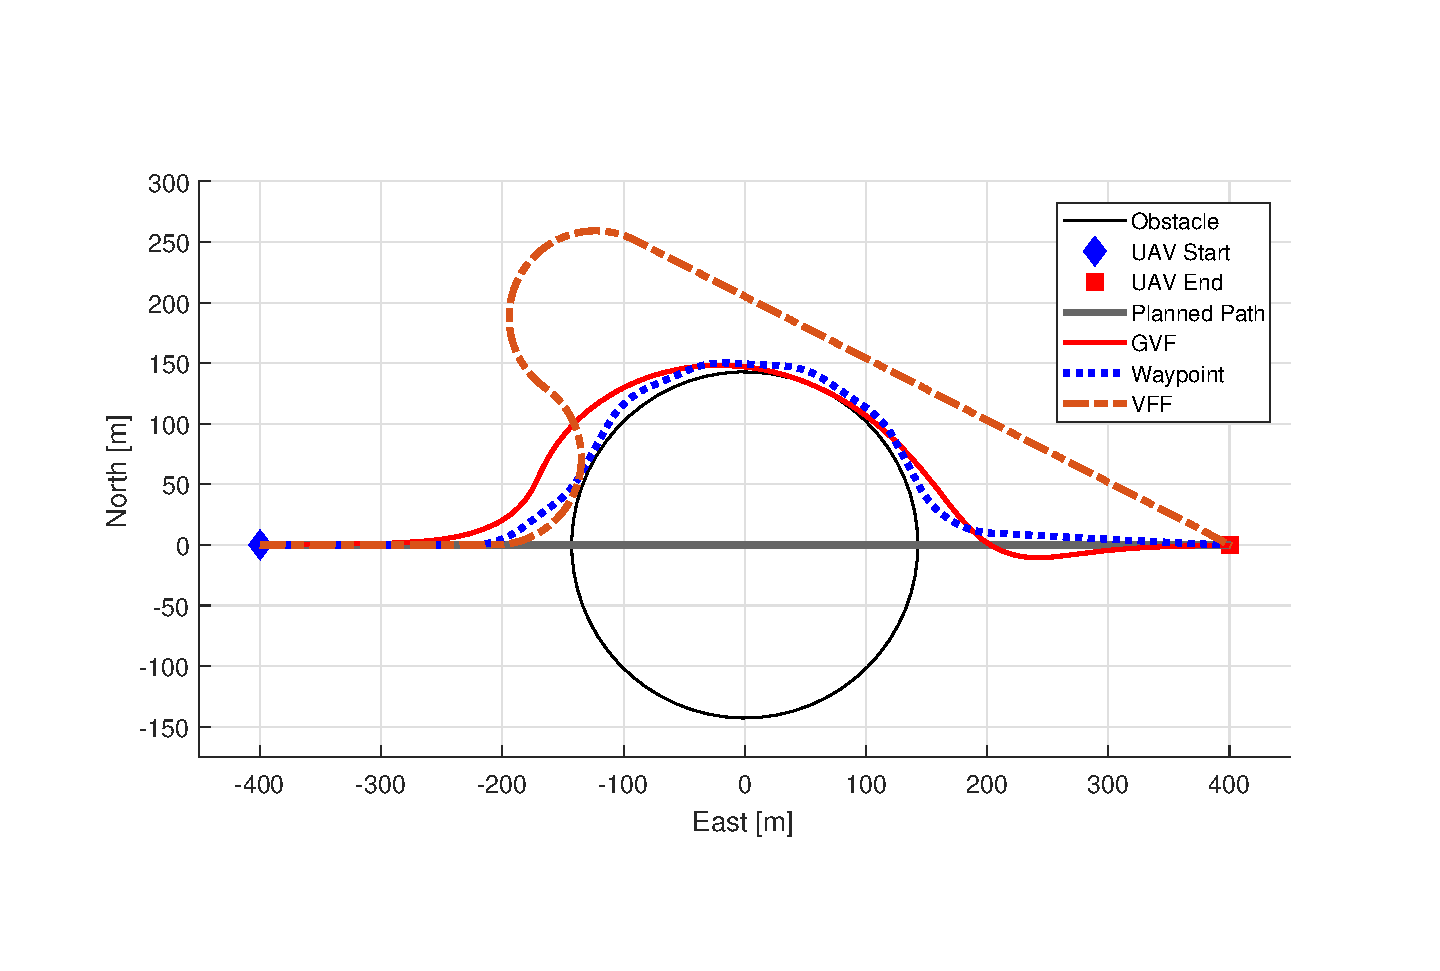
\includegraphics[trim=0 50 0 65,clip,width=15cm]{Figures/Simulations/compareMethods}
	\caption{Path of UAV guided by guidance methods}
	\label{fig:comparemethods}
\end{figure}


\begin{figure}[H]
	\centering
	\label{fig:barPlotCost}
	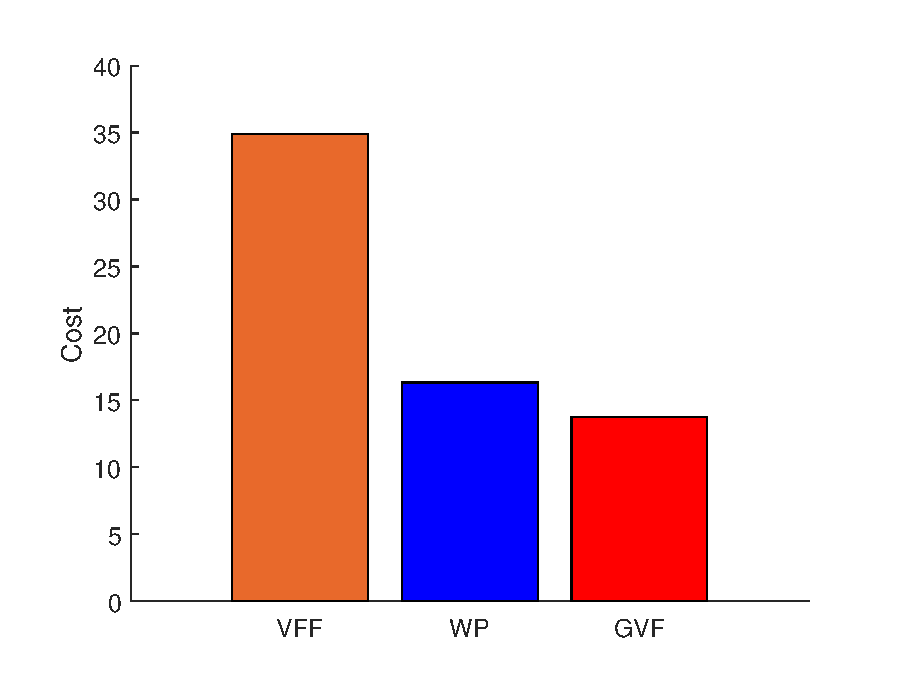
\includegraphics[width=15cm]{Figures/Simulations/barPlotPerformance}
	\caption{Cost performance for various UAV guidance methods}
	\label{fig:barplotperformance}
\end{figure}

A summary of the guidance methods cost and behavior that were simulated are shown in Table \ref{table}.

\begin{table}[H]
	\centering
	\caption{Obstacle Avoidance Method's Performance Summary }
	\label{table}
	\begin{tabular}{|l|c|c|c|}
		\hline
		\multicolumn{1}{|c|}{Method} & Cost {[}-{]} & Returns to path quickly & Avoids obstacle without replanning \\ \hline
		VFF                          & 31.8         &                         & \Checkmark
		\\ \hline
		GVF                          & 13.2         & \Checkmark                       & \Checkmark                                  \\ \hline
		WP                           & 12.7         & \Checkmark                       &                                    \\ \hline
	\end{tabular}
\end{table}





\section{Conclusion}
A gradient vector field for path following and circular obstacle avoidance was optimized and shown to have similar performance to waypoint avoidance without the need to re-plan the mission path. The obstacle avoidance GVF acts on the same principle as VFF, however guidance vectors are given circulation which aid in returning the UAV back to the planned path without intervention. Singularities in summed GVFs were identified by numerically finding locations where vector field magnitudes were null in a summed field. It was shown that optimizing circulation and decay radius of a repulsive GVF removed singularities from a UAVs path and reduced path deviation cost function by $150\%$ compared to VFF. Decay radius and circulation values were determined by minimizing a path deviation cost function. The improved GVF guidance was shown to have a reduced path deviation cost in comparison to potential field and traditional waypoint guidance. Increasing the number of deviation waypoints may provide guidance with lower cost than GVF, however when re-planning a path is not possible, such as instances where a ground station is not reachable, GVF provides a low cost method that can be computed on-board a UAV for avoiding obstacles without the need to re-plan the path. 



%The standoff tracking scenario in [wwc] did not address the possibility of attractive and repulsive vector fields canceling, leading to guidance singularities. Additionally, no method for determining the radius of the decay field was specified to minimize deviation from the planned path. A method for locating singularities in a summed vector field is presented, followed by an improved GVF for circular obstacle avoidance method. The improved GVF is compared in simulation to waypoint and potential field and it is shown to have favorable obstacle avoidance.
%
%
%
%
%
%Vector field guidance with optimized weights for avoiding obstacles and minimally deviating from a planned path was presented and compared to guidance methods in literature. Conventional methods for avoiding obstacles may require human intervention and require paths to be re-planned, such as waypoint navigation. Potential field eliminates the need for a path planner when encountering a new obstacle, however is not ideal for path following scenarios such as surveying a sensor line. Vector field guidance avoids re-planning and avoids an obstacle while returning to the original pre-planned path by selecting decay radius and circulation that minimizes a path deviation cost function. Singularities in the vector field are also avoided when circulation is added to the decay field. Future work to improve vector field for avoidance may include optimizing field parameters at each time step, potentially increasing time spent on the sensor line.

\bibliography{bib}

\end{document}
